\documentclass[a4paper,11pt]{article}
% Da man keine Unterst"utzung der deutschen Sprache in diesem Fall braucht!!
% \usepackage[german]{babel}

\setlength{\fboxrule}{.5mm}
\setlength{\fboxsep}{1.75mm}
\setlength{\footnotesep}{6pt}
\usepackage{hyperref}
\usepackage{amsmath}
\usepackage{amsfonts}
\usepackage{amsthm}
\usepackage{makeidx}
\usepackage[pdftex]{graphicx}
% \usepackage{graphicx}
\makeindex
\hypersetup{colorlinks=true}
\usepackage[flushmargin]{footmisc}

\setlength{\textwidth}{460 pt}
\hoffset-0.7in
\newtheorem{definition}{Definition}
%\newcommand{\href}[2]{#2}
\newcommand{\hypertag}[2]{#1}
%\newcommand{\hyperlink}[2]{#2}
%\newcommand{\hypertarget}[2]{#2}
\newtheorem{theorem}{Theorem}
\newenvironment{Proof}[1]
  {\textbf{Proof #1} \\}
  {\hfill$\Box$ \\}

%\pdfinfo{ /Title (CrypTool script)
%/Creator (TeX)
%/Producer (pdfTeX 0.14a)
%/Author (Deutsch Bank AG)
%/CreationDate (D:20000920201000)
%}


\title{ CrypTool Script \\ Mathematics and Cryptography }


\author{
(c) The authors, 1998-2002 \\
Frankfurt am Main
}

\begin{document}
\pagestyle{plain}
\setlength{\fboxrule}{.5mm}
\setlength{\fboxsep}{1.75mm}
\setlength{\footnotesep}{6pt}
\addtolength{\footskip}{8pt}
%\setlength{\footskip}{4cm}
%\renewcommand{\footnoterule}{\parindent0cm\rule{13cm}{.1pt}\vspace{.2cm}}
%Formatierung der Fu"snoten

%space between text and footnote 
\renewcommand\footnoterule{%
  \vspace{2em}%   <-- one line space between text and footnoterule
%\kern-3\p@
  \hrule width .4\columnwidth
 \vspace{4pt}
%kern 2.6\p@
}

%\long\def\@makefntext#1{%
%    \parindent 1em%
 %   \noindent
%    \hbox to 1.8em{\hss\@makefnmark}#1}

\maketitle

\parskip 4pt
\vskip + 30 pt
{
In this CrypTool script you will find predominantly mathematically oriented
information for using encryption procedures. The main chapters have been written
by {\em various authors} and are therefore independent from one another. At the end of
most chapters you will find literature and URLs.

You will receive information about the principles of symmetrical and
asymmetrical encryption. A large section of the script is dedicated to the
fascinating topic of prime numbers. Using numerous examples, the elementary number
theory and modular arithmetic are introduced and applied in an exemplary 
manner in the RSA procedure.  After this, one receives insight into the mathematical ideas
behind modern cryptography. 

%You will also obtain an overview of the
%mathematical ideas behind modern cryptography.

A further chapter is devoted to digital signatures, which are an essential
component of e-business applications. The last chapter --- elliptic curves ---
fits in well with this. The mathematics of elliptic curves forms the basis for
rapid cryptographic algorithms for digital signatures; these algorithms are
extremely well suited for implementation on smartcards.

Whereas the program CrypTool teaches you how to use cryptography in practice, the
script provides those interested in the subject with a deeper understanding of
the mathematical algorithms used -- trying to do it didactically as good as possible.

The {\em authors} Bernhard Esslinger, Bartol Filipovic, Henrik Koy and Roger Oyono
would like to take this opportunity to thank their colleagues in the company and
at the universities of Frankfurt, Giessen and Karlsruhe. They particularly thank
Dr. Peer Wichmann from the Karlsruhe computer science research centre
(Forschungszentrum Informatik, FZI) for his down-to-earth support.

\enlargethispage{0.5cm}
As at CrypTool, the quality of the script is enhanced through your suggestions
and ideas for improvement. We look forward to your feedback.


\vskip +7 pt \noindent
You will find the current version of CrypTool under \newline
  \href{http://www.CrypTool.de}{\tt http://www.CrypTool.de},~~
  \href{http://www.cryptool.com}{\tt http://www.CrypTool.com}~~ or~~
  \href{http://www.cryptool.org}{\tt http://www.CrypTool.org}.
{
\vskip + 7 pt \noindent
The contact persons for this free tool are listed in the readme file for
CrypTool.}
}


\newpage
\tableofcontents
\addcontentsline{toc}{section}{Contents}
\newpage
\normalsize
\parindent0cm
\parskip4pt

\section*{Introduction}  \addcontentsline{toc}{section}{Introduction}

This script is delivered together with CrypTool.

CrypTool is a program with an extremely comprehensive online help enabling you
to use and analyse cryptographic procedures.\par \vskip + 3pt

For the conventional encryption procedures, automatic analyses are available in CrypTool
that enable you to determine the key with knowledge of the encrypted document
and, possibly, further information (non-encrypted document or language of the
document).\par \vskip + 3pt

CrypTool was developed during the End-User Awareness program in order to
increase employee awareness of IT security and provide them with a deeper
understanding of the term security.\par \vskip + 3pt

A further aim was to enable users to understand the cryptographic procedures
implemented in the Deutsche Bank. In this way, using CrypTool as a reliable
reference implementation of the various encryption procedures (because of using the industry-proven SECUDE Library),
you can test the encryption implemented in other programs. \par \vskip + 3pt

Because the articles in this script are largely self-contained, this script can also
be read independantly of CrypTool.

The {\em authors} tried to describe cryptography for a broad audience --
without being mathematically incorrect. We believe, that this didactical pretention
is the way to promote the awareness for IT security and the readiness to use standardised modern cryptography.


\newpage
\section{Encryption procedures}

\subsection{Encryption}

The purpose of encryption \index{Encryption} is to change data in such a way
that only an authorised recipient is able to reconstruct the plaintext. This has
the advantage that you can transmit encrypted data openly and nevertheless need
not fear a perpetrator reading the data without authorisation. Authorised
recipients possess a piece of secret information --- called the key --- which
allows them to decrypt the data while it remains hidden from everyone else.\par \vskip + 3pt

One encryption procedure has been proved to be secure --- the {\em One-Time-Pad}.
\index{One�Time�Pad} However, this procedure has several practical
disadvantages (the key used must be selected randomly and must be just as long
as the message to be protected), which means that it is hardly used except in
closed environments such as for the hot wire between Moscow and Washington.\par \vskip + 3pt

For all other procedures there is a (theoretical) possibility of breaking them.
If the procedures are good, however, the time taken to break them is so long
that it is practically impossible to do and these procedures can therefore be
considered (practically) secure.\par \vskip + 3pt

We basically distinguish between symmetric and asymmetric encryption procedures.

\subsubsection{Symmetric encryption}

For {\em symmetric} encryption \index{Encryption!symmetric} the sender and
recipient must possess a common (secret) key which they have exchanged before
actually starting to communicate. The sender uses this key to encrypt the
message and the recipient uses it to decrypt it.\par \vskip + 3pt

The advantages of symmetric algorithms are the high speed with which data can be
encrypted and decrypted. One disadvantage is the need for key management. In
order to communicate with one another confidentially, sender and recipient must
have exchanged a key using a secure channel before actually starting to
communicate. Spontaneous communication between individuals who have never met
therefore seems virtually impossible. If everyone wants to communicate with
everyone else spontaneously at any time in a network of $ n $ subscribers, each
subscriber must have previously exchanged a key with each of the other $n-� 1$
subscribers. A total of $n(n - 1)/2$ keys must therefore be exchanged.\par \vskip + 3pt

The most well-known symmetric encryption procedure is the \index{DES} DES--
algorithm. The DES-algorithm has been developed by IBM in collaboration with the
National Security Agency \index{NSA} (NSA), and was published as a standard in
1975. Despite the fact that the procedure is relatively old, no effective attack
on it has yet been detected. The most effective way of attacking consists of
testing all possible keys until the right one is found ({\em brute--force--attack}).
\index{Attack!brute-force} Due to the relatively short key length of
effectively 56 bits (64 bits, which however include 8 parity bits), numerous
messages encrypted using DES have in the past been broken. Therefore, the
procedure can now only be considered to be conditionally secure. Symmetric
alternatives to the DES procedure include the IDEA \index{IDEA} or Triple DES
algorithms.\par \vskip + 3pt

Up-to-the-minute procedures are the symmetric AES procedures. The associated
Rijndael procedure was declared winner the AES award on 2 October 2000 and thus
succeeds the DES procedure.

\subsubsection{Asymmetric encryption}

In the case of {\em asymmetric} encryption \index{Encryption!asymmetric} each
subscriber has a personal pair of keys consisting of a {\em secret}
\index{Key!secret} key and a {\em public} key\index{Key!public}. The public
key, as its name implies, is made public, e.g. in a key directory on the
Internet.\par \vskip + 3pt

If Alice wants to communicate with Bob, then she finds Bob's public key in the
directory and uses it to encrypt her message to him. She then sends this
ciphertext to Bob, who is then able to decrypt it again using his secret key. As
only Bob knows his secret key, only he can decrypt messages addressed to him.
Even Alice who sends the message cannot restore plaintext from the (encrypted)
message she has sent. Of course, you must first ensure that the public key
cannot be used to derive the private key.\par \vskip + 3pt

Such a procedure can be demonstrated using a series of thief-proof letter boxes.
If I have composed a message, I then look for the letter box of the recipient
and post the letter through it. After that, I can no longer read or change the
message myself, because only the legitimate recipient possesses the key for the
letter box.\par \vskip + 3pt

The advantage of asymmetric procedures is the easy \index{Key
management} key management. Let's look again at a network with $n$
subscribers. In order to ensure that each subscriber can establish
an encrypted connection to each other subscriber, each subscriber
must possess a pair of keys. We therefore need $2n$ keys or $n$
pairs of keys. Furthermore, no secure channel is needed before
messages are transmitted, because all the information required in
order to communicate confidentially can be transmitted openly. In
this case, you simply have to pay attention to the accuracy
(integrity and authenticity) \index{Authenticity} of the public
key. Disadvantage: Pure asymmetric procedures take a lot longer to
perform than symmetric ones.\par \vskip + 3pt

The most well-known asymmetric procedure is the \index{RSA} RSA algorithm,
named after its developers Ronald \index{Rivest Ronald} Rivest, Adi
\index{Shamir Adi} Shamir and Leonard \index{Adleman Leonard} Adleman. The RSA algorithm
was published in 1978. The concept of asymmetric encryption was first
introduced by Whitfield Diffie \index{Diffie Whitfield}  and Martin
\index{Hellman Martin} Hellman in 1976. Today, the ElGamal \index{ElGamal}
procedures also play a decisive role, particularly the \index{Schnorr} Schnorr
variant in the \index{DSA} DSA (Digital \index{Signatures!digital}Signature
Algorithm).

\newpage
\subsubsection{Hybrid procedures}
\index{Hybrid procedures}
In order to benefit from the advantages of symmetric and asymmetric techniques
together, hybrid procedures are usually used (for encryption) in practice.\par \vskip + 3pt

In this case the data is encrypted using symmetric procedures: the key is a
session key generated by the sender randomly that is only used for this message.
This session key is then encrypted using the asymmetric procedure and
transmitted to the recipient together with the message. Recipients can determine
the session key using their secret keys and then use the session key to encrypt
the message. In this way, we can benefit from the easy key management \index{Key
management} of asymmetric procedures and encrypt large quantities of data
quickly and efficiently using symmetric procedures.

\subsubsection{Further details}

Beside information you can find in many books and on a lot of websites the online help
of CrypTool also offers very many details about the symmetric and asymmetric encryption methods.

\begin{thebibliography}{99999}
\addcontentsline{toc}{subsection}{Literatur}
\bibitem[Schmeh2001]{Schmeh2001}  \index{Schmeh 2001}
	Klaus Schmeh, \\
	Kryptografie und Public-Key Infrastrukturen im Internet, dpunkt.verlag, 2. akt. und erw. Auflage 2001. \\
	A considerable, up-to-date, good reading book, which considers practical problems, like standardisation or
	real existing software. Currently published only in German language.
\end{thebibliography}

%%%%%%%%%%%%%%%%%%%%%%%%%%%%%%%%%%%%%%%%%%%%%%%%%%%%%%%%%%%%%%%%%%%%%%%%%%
%
% C H A P T E R   T W O
%
%%%%%%%%%%%%%%%%%%%%%%%%%%%%%%%%%%%%%%%%%%%%%%%%%%%%%%%%%%%%%%%%%%%%%%%%%%

\newpage
\section{Prime numbers}\hypertarget{Kapitel_2}{}
(Bernhard Esslinger, besslinger@web.de, May 1999, Updates Nov. 2000, December 2001)

%\paragraph{What are prime numbers?}
\subsection*{What are prime numbers?}
\addcontentsline{toc}{subsection}{~~~~~~What are prime numbers?}
\index{Prime number} \index{Numbers!prime numbers}
Prime numbers are whole, positive numbers greater than or equal to $2$ that can
only be divided by 1 and themselves. All other natural numbers greater than or
equal to $2$ can be formed by multiplying prime numbers.

The {\em natural} \index{Numbers} numbers $\mathbb{N}=\{1, 2, 3, 4,\cdots \}$ thus comprise 
\begin{itemize}
   \item the number $1$ (the unit value)
   \item the primes and
   \item the composite numbers.
\end{itemize}

Prime numbers are particularly important for 3 reasons:
\begin{itemize}
  \item In number theory, they are considered to be the basic components of
natural numbers, upon which numerous brilliant mathematical ideas are based.
  \item They are of extreme practical importance in modern
\index{Cryptography!modern} cryptography (public key \index{Cryptography!public 
key} cryptography). The most common public key procedure, invented at the end of
the 1970's, is \index{RSA} RSA encryption. Only using (large) prime numbers for
particular parameters can you guarantee that an algorithm is secure, both for
the RSA procedure and for even more modern procedures (digital
\index{Signatures!digital} signature, elliptic curves).
  \item The search for the largest known prime numbers does not have any
practical usage known to date, but requires the best computers, is an excellent
benchmark (possibility for determining the performance of computers) and leads
to new calculation methods on many computers \\ (see also:
\href{http://www.mersenne.org/prime.htm}{\tt
http://www.mersenne.org/prime.htm}).
\end{itemize}
Many people have been fascinated by prime numbers over the past two millenniums.
Ambition to make new discoveries about prime numbers has often resulted in
brilliant ideas and conclusions. The following section provides an easily
comprehensible introduction to the basics of prime numbers. We will also explain
what is known about the distribution (density, number of prime numbers in
particular intervals) of prime numbers and how prime number tests work.

\subsection{Prime numbers in mathematics}

Every whole number has a factor. The number 1 only has one factor,
itself, whereas the number $12$ has the six factors $1, 2, 3, 4,
6, 12$. Many numbers can only be divided by themselves and by $1$.
With respect to multiplication, these are the ''atoms'' in the
area of numbers. Such numbers are called prime numbers.

In mathematics, a slightly different (but equivalent) definition is used.

\begin{definition}\label{def-pz-prime}
A whole number $p \in {\bf N}$ is called prime \index{Numbers!prime numbers} if
$p > 1$ and $p$ only possesses the trivial factors $\pm 1$ and $\pm p$.
\end{definition}


By definition, the number $1$ is not a prime number. In the following sections,
$p$ will always denote a prime number.

The sequence of prime numbers starts with $$ 2,~ 3,~ 5,~ 7, ~ 11, ~ 13, ~
17, ~ 19, ~ 23, ~ 29, ~ 31, ~ 37, ~ 41, ~ 43, ~ 47, ~ 53, ~ 59, ~ 61,
~ 67, ~ 71, ~ 73, ~ 79, ~ 83, ~ 89, ~ 97, \cdots . $$
The first 100 numbers include precisely 25 prime numbers. After this, the percentage of primes
constantly decreases. Prime numbers can be factorised in a unique {\em trivial}
way: $$5 = 1 \cdot 5,\quad  17 = 1 \cdot 17, \quad 1,013 = 1 \cdot 1,013,  \quad
1,296,409 = 1 \cdot 1,296,409.$$
All numbers that have $2$ or more factors are called \index{Numbers!composite}
{\em composite}. These include $$ 4 = 2 \cdot 2, \quad 6 = 2\cdot 3 $$ as well
as numbers that {\em look like primes}, but are in fact composite:
$$ 91 = 7 \cdot 13, \quad 161=7 \cdot 23, \quad 767 =13 \cdot 59. $$

\begin{theorem}\label{thm-pz-sqr}
Each whole number $m$ greater than $1$ possesses a lowest factor greater than
$1$. This is a prime number $p$. Unless $m$ is a prime number itself, then: $p$
is less than or equal to the square root of $m$.
\end{theorem}

All whole numbers greater than $1$ can be expressed as a product of prime
numbers --- in a unique way. This is the claim of the 1st fundamental theorem of
number theory (= fundamental theorem of arithmetic = fundamental building block
of all positive integers).

\begin{theorem}\label{thm-pz-prod}
Each element $n$ of the natural numbers greater than $1$ can be written as the
product $n = p_1 \cdot p_2 \dots p_m$ of prime numbers. If two such
factorisations $$n =  p_1 \cdot p_2 \cdots p_m = p'_1 \cdot p'_2 \cdots
p'_{m'}$$ are given, then they can be reordered such that $\;m = m'\;$ and for
all $i$:  $\;p_i = p'_i$.
\end{theorem}

In other words: each natural number other than $1$ can be written as a product
of prime numbers in precisely one way, if we ignore the order of the factors.
The factors are therefore unique (the {\em expression as a product of factors}
is unique)! For example, $$ 60 = 2 \cdot 2 \cdot 3 \cdot 5 = 2^2\cdot 3^1 \cdot
5^1. $$
And this --- other than changing the order of the factors --- is the only way in
which the number $60$ can be factorised. If you allow numbers other than primes
as factors, there are several ways of factorising integers and the uniqueness \hypertarget{uniqueness}{} is
lost: $$ 60 = 1 \cdot 60 = 2 \cdot 30 = 4 \cdot 15 = 5 \cdot 12 =6 \cdot 10 = 2
\cdot 3 \cdot 10 = 2 \cdot 5 \cdot 6 = 3 \cdot 4 \cdot 5 = \cdots . $$

The following section is aimed more at those familiar with mathematical logic:
The 1st fundamental theorem only appears to be obvious \label{remFundTheoOfArithm}. We can construct
numerous other sets of numbers (i.e. other than positive whole numbers greater
than 1), for which numbers in the set cannot be expressed uniquely as a product
of the prime numbers of the set: In the set $M = \{1, 5, 10, 15, 20, \cdots\}$
there is no equivalent to the fundamental theorem under multiplication. The
first five prime numbers of this sequence are $5, 10, 15, 20, 30$ (note: $10$ is
prime, because $5$ is not a factor of $10$ in this set --- the result is not an
element of the given basic set $M$). Because the following applies in $M$: $$
100 = 5 \cdot 20 = 10 \cdot 10 $$ and $5, 10, 20$ are all prime numbers in this
set, the expression as a product of prime factors is not unique here.

\subsection{How many prime numbers are there?}

For the natural numbers, the primes can be compared to elements in chemistry or
the elementary particles in physics (see \cite[p. 22]{Blum1999}).

Although there are only $92$ natural chemical elements, the number of prime
numbers is unlimited. Even the Greek, \index{Euclid} Euclid\footnote{Euclid,
a Greek mathematician of 4th and 3rd century before Christ. He worked at the
egyptian academy of Alexandria and wrote ''The Elements'', the most well known systematical textbook
of the Greek mathematics.} knew this in the
third century before Christ.
\begin{theorem}[Euclid]\label{thm-pz-euklid}\footnote{The common usage of the term does not denote Euclid as the inventor of the theorem rather;
the true inventor is merely not as prominent. The theorem has already been distinguished
and proven in Euclid�s Elements (Book IX, s. 20). The phraseology is remarkable due to 
the fact that the word infinite is not used. The text reads as following
$$
O\acute{\iota}~\pi\varrho\tilde{\omega}\tau o \iota~\grave{\alpha}\varrho\iota\vartheta\mu o\grave{\iota}~
\pi\lambda\varepsilon\acute{\iota}o \upsilon\varsigma~\varepsilon\grave{\iota}\sigma\grave{\iota}~
\pi\alpha\nu\tau\grave{o}\varsigma~\tau o \tilde{\upsilon}~
\pi\varrho o \tau\varepsilon\vartheta\acute{\varepsilon}\nu\tau o \varsigma~
\pi\lambda\acute{\eta}\vartheta\ o \upsilon\varsigma~
\pi\varrho\acute{\omega}\tau\omega\nu~
\grave{\alpha}\varrho\iota\vartheta\mu\tilde{\omega}\nu,
$$
the English translation of which is: the prime numbers are more than any previously existing amount
of prime numbers.}
The sequence of prime numbers does not discontinue.
Therefore, the quantity of prime numbers is infinite.
\end{theorem}
His proof that there is an infinite number of
primes is still considered to be a brilliant mathematical consideration and
conclusion today (proof by contradiction). He assumed that there is only a
finite number of primes and therefore a largest prime number. Based on this
assumption, he drew logical conclusions until he obtained an obvious
contradiction. This meant that something must be wrong. As there were no
mistakes in the chain of conclusions, it could only be the assumption that was
wrong. Therefore, there must be an infinite number of primes!

\hypertarget{euclid}{}
\paragraph{Euclid's proof by contradiction} argues as follows:

{\bf Assumption:} \quad There is a {\em finite} number of primes. \\*[4pt] {\bf
Conclusion:} \quad Then these can be listed $p_1 < p_2 < p_3 < \dots < p_n$,
where $n$ is the (finite) number of prime numbers. $p_n$ is therefore the
largest prime. Euclid now looks at the number $a = p_1 \cdot p_2 \cdots p_n +1$.
This number cannot be a prime number because it is not included in our list of
primes. It must therefore be divisible by a prime, i.e. there is a natural
number $i$ between $1$ and $n$, such that $p_i$ divides the number $a$. Of
course, $p_i$ also divides the product $a-1 = p_1 \cdot p_2 \cdots p_n$, because
$p_i$ is a factor of $a-1$. Since $ p_i $ divides the numbers $ a $ and $ a-1 $,
it also divides the difference of these numbers. Thus: $p_i$ divides  $a - (a-1)
= 1$. $p_i$ must therefore divide $1$, which is impossible. \\*[4pt] {\bf
Contradiction:} \quad Our assumption was false.

Thus there is an {\em infinite} number of primes
\hyperlink{primhfk}{(Cross-reference: overview under 2.6.1 of the number of
prime numbers in various intervals)}.\par \vskip + 3pt

Here we may mention yet another fact which is initially somewhat surprising. 
Namely, in the prime numbers sequence $p_1, p_2, \cdots,$ gaps between prime numbers can have
an individually determined length $n$. It is undeniable that under the $n$
succession of natural numbers
$$(n+1)!+2,\cdots, (n+1)!+(n+1),
$$
none of them is a prime number since in order, the numbers $2,3,\cdots,(n+1)$  
are comprised respectively as real divisors. 
($n!$ means the product of the first $n$ natural numbers therefore 
$ n!= n*(n-1)*\cdots *2*1$).

\subsection{The search for extremely large primes}

The largest prime numbers known today have several hundred
thousand digits, which is too big for us to imagine. The number of
elementary particles in the universe is ''only'' estimated to be a
$80$-digit number \hyperlink{grosord}{(See: overview under 2.6.3
of various orders of magnitude / dimensions)}.

Almost all known huge prime numbers are special candidates, called
\index{Mersenne Marin} {\em Mersenne numbers} of the form $2^p -1,$ where $p$ is
a prime. Marin Mersenne (1588-1648) was a French priest and mathematician. Not
all Mersenne numbers are prime:

$$
\begin{array}{cl}
2^2 - 1 = 3 & \Rightarrow {\rm prime} \\
2^3 - 1 = 7 & \Rightarrow {\rm prime} \\
2^5 - 1 = 31    & \Rightarrow {\rm prime} \\
   \vdots \\
2^{11} - 1 = 2.047 = 23 \cdot 89    & \Rightarrow  {\rm NOT~prime} !
\end{array}
$$

\index{Numbers!Mersenne numbers}\index{Mersenne Marin!Mersenne numbers}
\index{Mersenne Marin!theorem} Even Mersenne knew that not all Mersenne numbers
are prime (see exponent $p = 11$). A prime Mersenne number \index{Mersenne prime number} is called Mersenne prime number.  
However, he is to be thanked for the interesting conclusion that a number of the form $2^n-1$ is not a prime number
if $n$ is a composite number:

\begin{theorem}[Mersenne]\label{thm-pz-mersenne} If $2^n - 1$ is a prime number, then $n$ is also a
prime number.
\end{theorem}

\begin{Proof}{}
The theorem of Mersenne can be proved by contradiction. We therefore assume that
there exists a composite natural number $ n $ (with real factorisation)  $ n=n_1
n_2 $, with the property that $ 2^n -1 $ is a prime number.

From \begin{eqnarray*} (x^r-1)((x^r)^{s-1} + (x^r)^{s-2} + \cdots + x^r +1) & =
&  ((x^r)^s + (x^r)^{s-1} + (x^r)^{s-2} + \cdots + x^r) \\ &  & -((x^r)^{s-1} +
(x^r)^{s-2} + \cdots + x^r +1)  \\ & = & (x^r)^s -1 = x^{rs } -1,
\end{eqnarray*} we conclude \[ 2^{n_1 n_2} - 1 = (2^{n_1} -1)((2^{n_1})^{n_2 -1}
+ (2^{n_1})^{n_2 -2} + \cdots + 2^{n_1} + 1). \]
Because $ 2^n - 1 $ is a prime number, one of the above two factors on the
right-hand side must be equal to 1. This is the case if and only if $ n_1 =1 $
or $ n_2 =1$. But this contradicts our assumption. Therefore the assumption is
false. This means that there exists no composite number $ n, $ such that $ 2^n -
1 $ is a prime.
\end{Proof} \vskip + 5pt
Unfortunately this theorem only applies in one direction (the inverse does not
apply, no equivalence): see the above example $2^{11}-1, $ where $11$ is prime.

Mersenne claimed that $2^{67}-1$ is a prime number. There is also a mathematical
history behind this claim: it first took over 200 years before \index{Lucas
Edouard} Edouard Lucas (1842-1891) proved that this number is composite.
However, he argued indirectly and did not name any of the factors. Then Frank
Nelson showed in 1903 which factors make up this composite number: $$ 2^{67} -1
=147, 573, 952, 588, 676, 412, 927 = 193, 707, 721 \cdot 761, 838, 257, 287. $$
He admitted to having worked 20 years on the factorisation (expression as a
product of factors) of this 21-digit decimal number!

Due to the fact that the exponents of the Mersenne numbers do not use all
natural numbers, but only the primes, the {\em experimental space} is limited
considerably. The currently known Mersenne prime numbers \index{Mersenne prime number} 
have the exponents 
$$
\begin{array}{c}
2; ~ 3; ~ 5; ~ 7; ~ 13; ~ 17; ~ 19; ~ 31; ~ 61; ~ 89; ~ 107; ~ 127;
~ 521; ~ 607; ~ 1,279; ~ 2,203; ~ 2,281; ~ 3,217; ~ 4,253; ~ 4,423; \\
9,689; ~ 9,941, ~ 11,213; ~ 19,937; ~ 21,701; ~ 23,207; ~ 44,497; ~
86,243; ~ 110,503; ~ 132,049; ~ 216,091;\\
 756,839; ~ 859,433; ~ 1,257,787; ~ 1,398,269; ~ 2,976,221; ~ 3,021,377; ~
6,972,593; ~13,466,917.
\end{array}
$$
Thus $39$ Mersenne prime numbers are currently known.

The $19$th number with the exponent $4,253$ was the first with at least $1,000$ digits in  decimal system
(the mathematician Samual \index{Yates Samual} Yates coined the expression {\em
titanic} \index{Prime number!titanic} prime for this; it was discovered by
Hurwitz in 1961); the $27$th number with the exponent $44,497$ was the first
with at least $10,000$ digits in the decimal system (Yates coined the expression
\index{Prime number!gigantic}  {\em gigantic} prime for this. These names are
now long outdated).

The 37th number was found in January 1998 and has 909,526
digits in the decimal system, which corresponds to 33 pages in the newspaper!

\newpage
These numbers can be found at the following URLs:

{\href{http://reality.sgi.com/chongo/prime/prime_press.html}{\tt http://reality.sgi.com/chongo/prime/prime\_press.html}}
\vskip - 4pt \noindent
\begin{quote}
(The supercomputer manufacturer SGI Cray Research not only employed brilliant
mathematicians but also used the prime number tests as benchmarks for their
machines.)
\end{quote}
{\href{http://www.utm.edu/}{\tt http://www.utm.edu/}}
\vskip - 4pt \noindent
\begin{quote}
(At the university of Tennessee you will find extensive research results about
prime numbers.)
\end{quote}
\subsubsection{M-38 -- June 1999}\index{Mersenne Marin!M-38}
The 38th Mersenne prime, called M-38,
$$ 2^{6,972,593} - 1. $$
was discovered in June 1999 and has $2,098,960$ digits in the decimal system
(that corresponds to around 77 pages in the newspaper).

\subsubsection{M-39 -- December 2001} \index{Mersenne Marin!M-39}

The 39th Mersenne prime, called M-39, $$2^{13,466,917}-1,$$ was found at December 6, 2001 �- more exactly,
the verification of this number, found at November 14, 2001 by the Canadian student Michael Cameron,
was successfully finished. This number has about 4 million decimal digits (exactly 4,053,946 digits).
Trying only to print this number $(924947738006701322247758 \cdots 1130073855470256259071)$ in the Financial Times
would need around 200 pages.

\subsubsection{GIMPS}\index{GIMPS}

Discovering the 39th Mersenne prime the GIMPS project (Great Internet Mersenne Prime Search) founded in 1996
already discovered for the 5th time the greatest Mersenne number to be proven being prime.

Now more than 130,000 volunteers, amateurs and experts, are working for the GIMPS project. They connect their
computers into the so called ''primenet'', organized by the company entropia, to find such numbers using distributed
computer programs.

\subsubsection{EFF}\index{EFF}

This search is also spurred on by a competition started by the non-profit
organisation EFF (Electronic Frontier Foundation) using the means of an unknown
donator. The participants are rewarded with a total of 500,000 USD if they find
the longest prime number. In promoting this project, the unknown donator is not
looking for the quickest computer, but rather wants to draw people's attention
to the possibilities offered by {\em cooperative networking}

{\href{http://www.eff.org/coopawards/prime-release1.html}{\tt http://www.eff.org/coopawards/prime-release1.html}}.

The discoverer of M-38 got for discovering the first prime with more than 1 million decimal digits 50,000 USD
from the EFF. The next price from EFF with 100,000 USD is for a proven prime with more than 10 million decimal digits.
%{\href{http://www.octocad.demon.co.uk/mersenne/prime.htm }{\tt http://www.octocad.demon.co.uk/mersenne/prime.htm}}.

Edouard Lucas (1842-1891) held the record for the longest prime number for over
70 years by proving that $2^{127}-1$ is prime. No new record is likely to last
that long.

\subsubsection{Prime number tests}
\index{Prime number!test}
In order to implement secure encryption procedures we need extremely large prime
numbers (in the region of $2^{2,048}$, i.e. numbers with $600$ digits in the
decimal system!).

Up to now we have always looked for the prime factors in order to decide whether
a number is prime. However, if even the smallest prime factor is enormous, the
search takes too long. Factorising numbers using systematic computational
division or using the sieve of Eratosthenes (see below) is only feasible using
current computers for numbers with up to around $20$ digits in the decimal
system.

However, if we know something about the {\em construction} of the number in
question, there are extremely highly developed procedures that are much quicker.
In the 17th century, Fermat wrote to Mersenne that he presumed that all numbers
of the form $$ F(n) = 2^{2^n} + 1 $$ are prime for all whole numbers $n$ greater
than or equal to $0$ (see below).

As early as in the 19th century, it was discovered that the $29$-digit number $$
F(7) = 2^{2^7} + 1 $$ is not prime. However, it was not until 1970 that
Morrison/Billhart managed to factorise it.
\begin{eqnarray*}
F(7) & = & 34,279,974,696,877,740,253,374,607,431,768,211,457 \\
& = & 59, 649, 589, 127, 497, 217 \cdot  574, 689, 200, 685,
129,054, 721.
\end{eqnarray*}
Many rapid prime number tests are based on the (small) Fermat theorem put
forward by Fermat in 1640 .
\index{Fermat!small Fermat}
\begin{theorem}[''small'' Fermat]\label{thm-pz-fermat1}
Let $p$ be a prime number and $a$ be any whole number, then for all $a$ $$a^p
\equiv a \; {\rm mod} \; p.$$
This could also be formulated as follows: \\ Let $p$ be a prime number and $a$
be any whole number that is not a multiple of $p$ (also $a \not\equiv 0 \; {\rm
mod} \; p$), then $a^{p-1} \equiv 1 \; {\rm mod} \; p$.
\end{theorem}

If you are not used to calculating with remainders (modulo), please simply
accept the theorem. What is important here is that this sentence implies that if
this equation is not met for any whole number $a$, then $p$ is not a prime! The
tests (e.g. for the first formulation) can easily be performed using the {\em
test basis} $a = 2$.

This gives us a criterion for non-prime numbers, i.e. a negative test, but no
proof that a number $a$ is prime. Unfortunately Fermat's theorem does not apply
--- otherwise we would have a simple proof of the prime number property (or to
put it in other words, we would have a simple prime number criterion).

Comment: Numbers that have the property $$ 2^n \equiv 2 \;{\rm mod}\; n $$ but
are not prime are called \index{Pseudoprime number}\index{Numbers!pseudoprime
number} {\em pseudoprime numbers}. The first pseudoprime number (i.e. not a
prime) is $$ 341 = 11 \cdot 31. $$
There are numbers that pass the Fermat test with all bases and yet are not
prime: these numbers are called \index{Numbers!Carmichael numbers} {\em
Carmichael numbers}. The first of these is $$ 561 = 3 \cdot 11 \cdot 17. $$
A stronger test is provided by \index{Miller} \index{Rabin} Miller/Rabin: it is
only passed by so-called {\em strong pseudoprime numbers}. Again, there are
strong pseudoprime numbers that are not primes, but this is much less often the
case than for (simple) pseudoprime numbers. The smallest strong pseudoprime
number base $2$ is $$ 15,841 = 7 \cdot 31 \cdot 73. $$
If you test all 4 bases, $2, 3, 5$ and $7$, you will find only one strong
pseudoprime number up to $25 \cdot 10^9$, i.e. a number that passes the test and
yet is not a prime number.

More extensive mathematics behind the Rabin test delivers the probability that
the number examined is prime (such probabilities are currently around $10^{-
60}$).

Detailed descriptions of tests for finding our whether a number is prime can be
found on Web sites such as:

{\href{http://www.utm.edu/research/primes/mersenne.shtml}{\tt
http://www.utm.edu/research/primes/mersenne.shtml}} and

{\href{http://www.utm.edu/research/primes/prove/index.html}{\tt
http://www.utm.edu/research/primes/prove/index.html}}.



\subsection{The search for a formula for prime numbers}
\index{Prime number!formula}
There are currently no useful, open (i.e. not recursive) formulae known that
only deliver prime numbers (recursive means that in order to calculate the
function the same function is used with a smaller variable). Mathematicians
would be happy if they could find a formula that leaves gaps (i.e. does not
deliver all prime numbers) but does not deliver any composite (non-prime)
numbers.

Ideally, we would like, for the number $n$, to immediately obtain the $n$-th
prime number, i.e. for $f(8) = 19\,$ or for  $f(52) = 239$.

Ideas for this can be found at

{\href{http://www.utm.edu/research/primes/notes/faq/p_n.html}
 {\tt http://www.utm.edu/research/primes/notes/faq/p\_n.html}}.


Cross-reference:  \hyperlink{ntePrimzahl}{the table under 2.6.2} contains the precise values for the $n$th
prime numbers for selected $ n.$

The following are some of the most common ideas for prime number formulae:
\begin{enumerate}
  \item Mersenne numbers  $f(n) = 2^n - 1$: \\
    As shown above, this formula seems to deliver relatively large prime numbers
but - as for $n=11$ [$f(n)=2,047$] - it is repeatedly the case that the result
is not prime.
  \item $F(k,n) = k \cdot 2^n \pm 1$  for $ n $ prime and $ k $ small primes:\\
   For this generalisation of the Mersenne numbers there are (for small $k$)
also extremely quick prime number tests (see \cite{Knuth1981}). This can be
performed in practice using software such as the PROTHS software from Yves
Gallot

({\href{http://www.prothsearch.net/index.html}{\tt
http://www.prothsearch.net/index.html}}).

  \item {\em Fermat numbers}\footnote{The Fermat prime numbers play a role in circel division.
As proven by Gauss\index{Gauss}, a regular $p$-edge
can only be constructed with the use of a pair of compasses and a ruler, when $p$ is a Fermat prime number.}
\index{Numbers!Fermat numbers}\index{Fermat!Fermat
number}  $F(n) = 2^{2^n} + 1$:\\
As mentioned above, Fermat wrote to Mersenne regarding this assumption.
Surprisingly he would have been able obtain a positive result using the negative
prime number test for $n=5$ based on his small theorem.
$$
\begin{array}{lll}
F(0) = 2^{2^0} + 1  = 2^1 + 1 & = 3 &   \mapsto {\rm ~prime}  \\
F(1) = 2^{2^1} + 1  = 2^2 + 1 & = 5 &   \mapsto {\rm ~prime}  \\
F(2) = 2^{2^2} + 1  = 2^4 + 1 & = 17 &  \mapsto {\rm ~prime}  \\
F(3) = 2^{2^3} + 1  = 2^8 + 1 & = 257 & \mapsto {\rm ~prime}  \\
F(4) = 2^{2^4} + 1  = 2^{16} + 1 &  = 65,537 &  \mapsto {\rm ~prime}  \\
F(5) = 2^{2^5} + 1  = 2^{32} + 1 &  = 4 ,294, 967, 297 = 641 \cdot
6,700,417 &  \mapsto {\rm ~NOT~prime} !
\end{array} 
$$
  \item Carmichael numbers: see above.
  \item Pseudoprime numbers: see above.
  \item Strong pseudoprime numbers: see above.
  \item Idea based on \hyperlink{euclid}{Euclid's proof} (infinite many prime
numbers) $p_1 \cdot p_2 \cdots p_n +1$:

$$
\begin{array}{lll}
2{\cdot}3 +1 &      = 7 &          \mapsto {\rm ~prime} \\
2{\cdot}3{\cdot}5 +1 &      = 31    &      \mapsto {\rm ~prime} \\
2{\cdot}3{\cdot}5{\cdot}7 +1 &      = 211   &      \mapsto {\rm ~prime} \\
2{\cdot}3{\cdots}11 +1 &        = 2,311  &      \mapsto {\rm ~prime} \\
2\cdot3 \cdots 13 +1 &  = 59 \cdot 509 &    \mapsto {\rm ~NOT~prime} ! \\
2\cdot3 \cdots 17 +1 &  = 19 \cdot 97 \cdot 277 &   \mapsto {\rm ~NOT~prime} !
\\
\end{array}
$$

  \item As above but except $+1$: $p_1 \cdot p_2 \cdots p_n -1$

$$
\begin{array}{lll}
2\cdot 3 -1     &   = 5 &   \mapsto {\rm ~prime} \\
2\cdot 3 \cdot  5  -1   &   = 29 &  \mapsto {\rm ~prime} \\
2\cdot 3 \cdots 7  -1   &   = 11 \cdot 19 & \mapsto {\rm ~NOT~prime} ! \\
2\cdot 3 \cdots 11 -1   &   = 2,309 &    \mapsto {\rm ~prime} \\
2\cdot 3 \cdots 13 -1   &   = 30,029 &    \mapsto {\rm ~prime} \\
2\cdot 3 \cdots 17 -1    &  = 61 \cdot 8,369 &   \mapsto {\rm ~NOT~prime!}
\end{array} 
$$

  \item \index{Euclidean number} {\em Euclidean numbers} $e_n = e_0 \cdot e_1
\cdots e_{n-1} + 1$  with $n$ greater than or equal to $1$ and $e_0 := 1$.
$e_{n-1}$ is not the $(n-1)$th prime number, but the number previously found
here.
    Unfortunately this formula is not open but recursive.
    The sequence starts with 

$$
 \small\begin{array}{lll}
e_1 = 1 + 1 &   = 2 &   \mapsto {\rm ~prime} \\
e_2 = e_1 + 1   &   = 3 &   \mapsto {\rm ~prime} \\
e_3 = e_1 \cdot e_2 + 1 &   = 7 &   \mapsto {\rm ~prime} \\
e_4 = e_1 \cdot e_2 \cdot e_3 + 1 & = 43 &  \mapsto {\rm ~prime} \\
e_5 = e_1 \cdot e_2 \cdots e_4 + 1 &    = 13 \cdot 139 &    \mapsto {\rm
~NOT~prime} ! \\
e_6 = e_1 \cdot e_2 \cdots e_5 + 1 &    = 3,263,443 &   \mapsto {\rm ~prime} \\
e_7 = e_1 \cdot e_2 \cdots e_6 + 1 &    = 547 \cdot 607 \cdot 1,033 \cdot 31,051
& \mapsto {\rm ~NOT~prime} ! \\
e_8 = e_1 \cdot e_2 \cdots e_7 + 1 &    = 29,881\cdot 67,003 \cdot 9,119,521
\cdot 6,212,157,481 & \mapsto {\rm ~NOT~prime} !
\end{array} 
$$

$e_9, \cdots, e_{17}$ are also composite, which means that this formula is not
particularly useful. Comment: However, what is special about all these numbers
is that any pair of them does not have a common factor other than $1$. They are
therefore \index{Prime number!relative} {\em relatively prime }.
  \item $f(n) = n^2 + n + 41$:\\
  This sequence starts off very {\em promisingly},   but is far from being a
proof.

$$
 \begin{array}{ll}
f(0) = 41 & \mapsto {\rm ~prime} \\
f(1) = 43 & \mapsto {\rm ~prime} \\
f(2) = 47 & \mapsto {\rm ~prim} \\
f(3) = 53 & \mapsto {\rm ~prime} \\
f(4) = 61 & \mapsto {\rm ~prime} \\
f(5) = 71 & \mapsto {\rm ~prime} \\
f(6) = 83 & \mapsto {\rm ~prime} \\
f(7) = 97 & \mapsto {\rm ~prime} \\
\vdots \\
f(39) = 1,601 & \mapsto {\rm ~prime} \\
f(40) = 11 \cdot 151 &  \mapsto {\rm ~NOT~prime}! \\
f(41) = 41 \cdot 43 &   \mapsto {\rm ~NOT~prime}! \\
\end{array} 
$$

The first $40$ values are prime numbers (which have the obvious regularity that
their difference starts with $2$ and increases by $2$ each time), but the $41$th
and $42$th values are not prime numbers.     It is easy to see that $f(41)$ hl
cannot be a prime number:
    $f(41) = 41^2 + 41 + 41 = 41 (41 + 1 + 1) = 41 \cdot 43$.
  \item $f(n) = n^2 - 79 \cdot n + 1,601$: \\
    This function delivers prime numbers for all values from $n=0$ to $n=79$.
Unfortunately $f(80) = 1,681 = 11 \cdot 151$ is not a prime number. To this
date, no function has been found that delivers more prime numbers in a row. On
the other hand, each prime occurs twice (first in the decreasing then in the
increasing sequence), which means that the algorithm delivers a total of 40
difference prime values (the same ones as the function from point 10).
$$
\begin{array}{|ll||ll|}
\hline
f(0) = 1,601    & \mapsto {\rm ~prime} &  f(28) = 173    & \mapsto {\rm ~prime}
\\
f(1) = 1,523    & \mapsto {\rm ~prime} &  f(29) = 151    & \mapsto {\rm ~prime}
\\
f(2) = 1,447    & \mapsto {\rm ~prime} &  f(30) = 131 & \mapsto {\rm ~prime} \\
f(3) = 1,373    & \mapsto {\rm ~prime} &  f(31) = 113 & \mapsto {\rm ~prime} \\
f(4) = 1,301    & \mapsto {\rm ~prime} &  f(32) = 97 & \mapsto {\rm ~prime} \\
f(5) = 1,231    & \mapsto {\rm ~prime} &  f(33) = 83 & \mapsto {\rm ~prime} \\
f(6) = 1,163    & \mapsto {\rm ~prime} &  f(34) = 71 & \mapsto {\rm ~prime} \\
f(7) = 1,097    & \mapsto {\rm ~prime} &  f(35) = 61 & \mapsto {\rm ~prime} \\
f(8) = 1,033    & \mapsto {\rm ~prime} &  f(36) = 53 & \mapsto {\rm ~prime} \\
f(9) = 971  & \mapsto {\rm ~prime} &  f(37) = 47 & \mapsto {\rm ~prime} \\
f(10) = 911 & \mapsto {\rm ~prime} &  f(38) = 43 & \mapsto {\rm ~prime} \\
f(11) = 853 & \mapsto {\rm ~prime} &  f(39) = 41 & \mapsto {\rm ~prime} \\
f(12) = 797 & \mapsto {\rm ~prime} &             &                     \\
f(13) = 743 & \mapsto {\rm ~prime} &  f(40) = 41 & \mapsto {\rm ~prime} \\
f(14) = 691 & \mapsto {\rm ~prime} &  f(41) = 43 & \mapsto {\rm ~prime} \\
f(15) = 641 & \mapsto {\rm ~prime} &  f(42) = 47 & \mapsto {\rm ~prime} \\
f(16) = 593 & \mapsto {\rm ~prime} &  f(43) = 53 & \mapsto {\rm ~prime} \\
f(17) = 547 & \mapsto {\rm ~prime} &  \cdots  &  \\
f(18) = 503 & \mapsto {\rm ~prime} &  f(77) = 1,447  & \mapsto {\rm ~prime} \\
f(19) = 461 & \mapsto {\rm ~prime} &  f(78) = 1,523  & \mapsto {\rm ~prime} \\
f(20) = 421 & \mapsto {\rm ~prime} &  f(79) = 1,601  & \mapsto {\rm ~prime} \\
f(21) = 383 & \mapsto {\rm ~prime} &  f(80) = 11 \cdot 151 & \mapsto {\rm
~NOT~prime!} \\
f(22) = 347 & \mapsto {\rm ~prime} &  f(81) = 41 \cdot 43 & \mapsto {\rm
~NOT~prime!} \\
f(21) = 383 & \mapsto {\rm ~prime} &  f(82) = 1,847  & \mapsto {\rm ~prime} \\
f(22) = 347 & \mapsto {\rm ~prime} &  f(83) = 1,933  & \mapsto {\rm ~prime} \\
f(23) = 313 & \mapsto {\rm ~prime} &  f(84) = 43 \cdot 47 &  \mapsto {\rm
~NOT~prime!} \\
f(24) = 281 & \mapsto {\rm ~prime} & & \\
f(25) = 251 & \mapsto {\rm ~prime} & & \\
f(26) = 223 & \mapsto {\rm ~prime} & & \\
f(27) = 197 & \mapsto {\rm ~prime} & & \\
\hline
\end{array} 
$$
  \item Polynomial functions $f(x) = a_n x^n + a_{n-1}x^{n-1} + \cdots + a_1 x^1 +
a_0$  ($a_i$ in ${\mathbb Z}$, $n \geq 1$):

    There exists no such polynomial that for all $x$ in ${\mathbb Z}$ only
delivers prime values.
    For a proof of this, please refer to \cite[p. 83 f.]{Padberg1996}, where you
will also find further details about prime number formulae.
  \item  \index{Catalan numbers} Catalan, after whom the so-called
{\em Catalan numbers} $A(n) = (1 / (n+1) ) * (2n)! / (n!)^2$ are named,
conjectured that $C_4$ is a prime:
$$
 \begin{array}{l}
C_0 = 2, \\
C_1 = 2^{C_0} - 1,  \\
C_2 = 2^{C_1} - 1,  \\
C_3 = 2^{C_2} - 1, \\
C_4 = 2^{C_3} - 1, \cdots \\
\end{array}
$$
    (see {\href{http://www.utm.edu/research/primes/mersenne.shtml}{\tt
http://www.utm.edu/research/primes/mersenne.shtml}} under Conjectures and
Unsolved Problems).

    This sequence is also defined recursively and increases extremely quickly.
Does it only consist of primes?
$$
\begin{array}{lll}
C(0) = 2 & & \mapsto {\rm ~prime}\\
C(1) = 2^2 - 1 &    = 3 & \mapsto {\rm ~prime}\\
C(2) = 2^3 - 1 &    = 7 & \mapsto {\rm ~prime} \\
C(3) = 2^7 - 1 &    = 127& \mapsto {\rm ~prime} \\
C(4) = 2^{127} - 1 &      = 170, 141, 183, 460, 469, 231, 731, 687, 303, 715,
884, 105, 727 & \mapsto {\rm ~prime} \\
\end{array} 
$$
It is not (yet) known whether $C_5$ and higher elements are prime, but this is
not very likely.
In any case, it has not been proved that this formula delivers only primes.
\end{enumerate}


\subsection{Density and distribution of the primes}

As Euclid discovered, there is an infinite number of primes. However, some
infinite sets are {\em denser} \index{Prime number!density} than others. Within
the set of natural numbers, there is an infinite number of even, uneven and
square numbers.

The following proves that there are more even numbers than square ones:
\begin{itemize}
  \item the size of the $n$th element: \\
    The $n$th element of the even numbers is $2n$; the $n$th element of the
square numbers is $n^2$. Because for all $n>2$: $2n < n^2$, the $n$th even
number occurs much earlier than the $n$th square number.
    Thus the even numbers are distributed more densely and we can say that there
are more even numbers than square ones.
  \item the number of values that are less than or equal to a certain {\em
maximum value} $x$ in ${\mathbb R}$ is: \\
    There are $[x/2]$ such even numbers and $[\sqrt{x}]$ square numbers. Because
for large $x$ the value $x/2$ is much greater than the square root of $2$, we
can again say that there are more even numbers.
\end{itemize}
\vskip +3 pt
\begin{theorem}\label{thm-pz-density}
For large n: The value of the $n$th prime $P(n)$ is asymptotic to $n \cdot
ln(n)$, i.e. the limit of the relation  $P(n)/(n\cdot \ln n)$ is equal to $1$ if
$n$ tends to infinity.
\end{theorem}


The definition is similar for the number of prime numbers $PI(x)$
that do not exceed the maximum value $x$:

\begin{theorem}\label{thm-pz-pi-x}
$PI(x)$  is asymptotic to  $x / ln(x)$.
\end{theorem}


This is the \index{Prime number!theorem} \textbf{prime number theorem}. It was
put forward by Legendre \index{Legendre} (1752-1833) and Gauss\index{Gauss} (1777-1855) but not proved until
over 100 years later.

\hyperlink{primhfk}{(Cross-reference: overview under 2.6.1 of the number of
prime numbers in various intervals).}

For large $n$, $P(n)$  lies between  $2n$  and  $n^2$. This means that there are
fewer primes numbers than even natural numbers but more prime numbers than
square numbers.

These formulae, which only apply when n tends to infinity, can be replaced by
more precise formulae.
For $x \geq 67$:
$$ ln(x) - 1,5 < x / PI(x) < ln(x) - 0,5 $$
As we know that $PI(x)  =  x / \ln x$ only for very large $x$ ($x$ tending
towards infinity), we can create the following overview:
$$
\begin{array}{ccccc}
x     &  ln(x)  &  x / ln(x) & PI(x)(counted) &       PI(x) / (x/ln(x)) \\
10^3  &  6.908  &   144      &  168        &       1.160 \\
10^6  &  13.816 &   72,386    &  78,498          &       1.085 \\
10^9  & 20.723  &   48,254,942 &  50,847,534       &       1.054
\end{array}
$$

For a binary number (number in the binary system) of the length $250$ bits
($2^{250}$ is approximately = $1.809 251 * 10^{75}$): $$ PI(250) = 2^{250} /
(250 \cdot \ln 2) \; {\rm is~approximately} \; =  2^{250} /173.28677 = 1.045 810
\cdot 10^{73}. $$
We can therefore expect that the set of numbers with a bit length of less than
250 contains approximately $10^{73}$ primes (a reassuring result?!).

We can also express this as follows: Let us consider a {\em random} natural
number $n$. Then the probability that this number is prime is around $1 / \ln(n)$.
For example, let us take numbers in the region of $10^{16}$. Then we must
consider $ 16 \cdot \ln 10 = 36,8 $ numbers (on average) until we find a prime.
A precise investigation shows: There are $10$ prime numbers between $10^{16}-
370$ and $10^{16}-1$.

Under the heading {\em How Many Primes Are There} under

{\href{http://www.utm.edu/research/primes/howmany.shtml}{\tt
http://www.utm.edu/research/primes/howmany.shtml}}.

you will find numerous other details.

Using the following Web site:

{\href{http://www.math.Princeton.EDU/~arbooker/nthprime.html}{\tt
http://www.math.Princeton.EDU/\~{}arbooker/nthprime.html}}

you can easily determine $PI(x)$.


The \textbf{distribution} of primes displays several irregularities for which no
�system� has yet been found. (On the one hand, many occur closely together, like
$2$ and $3,$ $ 11$ and $13, $ $ 809$ and $811$, on the other hand large gaps
containing no primes also occur. For example, no primes lie between $113$ and
$127, $ $ 293$ and $307, $ $317$ and $331, $ $ 523$ and $541, $ $ 773$ and $787,
$ $ 839$ and $853$ as well as between $887$ and $907$) (For details, see:

{\href{http://www.utm.edu/research/primes/notes/gaps.html}{\tt
http://www.utm.edu/research/primes/notes/gaps.html}}).

This is precisely part of what motivates mathematicians to discover its secrets.
\index{Eratosthenes!sieve}
\paragraph{Sieve of Eratosthenes}
An easy way of calculating all $PI(x)$ primes less than or equal to $x$ is to
use the sieve of Eratosthenes. In the 3rd century before Christ, he found an
extremely easy, automatic way of finding this out. To begin with, you write down
all numbers from 2 to $x$, circle 2, then cross out all multiples of 2. Next,
you circle the lowest number that hasn't been circled or crossed out (3) and
again cross out all multiples of this number, etc. You only need to continue
until you reach the largest number whose square is less than or equal to $x$.

Apart from 2, prime numbers are never even. Apart from 2 and 5, prime numbers
never end in 2, 5 or 0. So you only need to consider numbers ending in 1, 3, 7,
9 anyway (there are infinite primes ending in these numbers; see \cite[vol. 1,
p. 137]{Tietze1973}).

You can now find a large number of finished programs on the Internet - often
complete with source code - allowing you to experiment with large numbers
yourself. You also have access to large databases that contain either a large
number of primes or the factorisation of numerous composite numbers. The
\index{Cunningham project} \textbf{Cunningham project} for example, determines
the factors of all composite numbers that are formed as follows: $$ f(n) = b^n
\pm 1  \quad {\rm for~} b = 2, 3, 5, 6, 7, 10, 11, 12 $$ ($b$ is not equal to
multiples of bases already used, such as $4, 8, 9$).

Details of this can be found under:

{\href{http://www.cerias.purdue.edu/homes/ssw/cun}{\tt
http://www.cerias.purdue.edu/homes/ssw/cun}}

\subsection{Notes}

\textbf{Proven statements / theorems about primes}

\begin{itemize}
  \item For each number $n$ in ${\bf N}$ there are $n$ consecutive natural
numbers that are not primes.
    A proof of this can be found in \cite[p. 79]{Padberg1996}.
  \item The Hungarian mathematician Paul Erd\"os (1913-1996) proved:
    Between each random number not equal to $1$ and its double, there is at
least one prime. (He was not the first to prove this theorem, but proved it in a
simpler manner than those before him).
  \item There is a real number a such that the function $f: {\bf N} \rightarrow
{\mathbb Z}$ where $n \mapsto a^{3^n}$     only delivers primes for all $n$ (see
\cite[p. 82]{Padberg1996}).
    Unfortunately, problems arise when we try to determine $a$ (see below).
\end{itemize}

\textbf{Proven statements / conjectures about primes}

\begin{itemize}
  \item The German mathematician \index{Goldbach Christian} Christian Goldbach
(1690-1764) conjectured:
    Every even natural number greater than 2 can be represented as the sum of
two prime numbers.
    Computers have verified\footnote{It is generally accepted today, that
the Goldbach Conjecture is true, i.e. valid for all even natural numbers bigger than $2$.
In 1999, mathematician J\"org Richtstein from the computer sciences institute at the University
of Giessen, studied even numbers up to 400 billion and found no contradictory example (see
\href{http://www.informatik.uni-giessen.de/staff/richstein/de/Goldbach.html}{\tt http://www.informatik.uni-giessen.de/staff/richstein/de/Goldbach.html}).\index{Richstein 1999}
Nevertheless, this does not provide us with general proof.\\
The fact that despite all efforts, Goldbachs' conjecture has to date not been proven leads
one to believe that: since the pioneer work of the Austrian mathematician Kurt G\"odel \index{G\""odel Kurt} is well-known,
not every true mathematical theorem is provable (see
\href{http://www.mathematik.ch/mathematiker/goedel.html}{http://www.mathematik.ch/mathematiker/goedel.html}).
Perhaps Goldbachs' Conjecture was correct, despite that however,
proof will never be found. Conversely, that will presumably also remain unproven.}
the Goldbach conjecture for all even numbers up to
$4*10^{14}$ but no general proof has yet been found\footnote{The English
publisher {\em Faber} and the American publisher {\em Bloomsbury} issued in 2000
the 1992 published book ''Uncle Petros and Goldbach's Conjecture'' by Apostolos Doxiadis.
It's the story of an old maths professor who fails to prove a more than 250 old puzzle. To
stimulate the sell rates the English and American publisher compete a prize of 1 million USD, 
is someone proves the conjecture -- to be published till 2004 by an well-known mathematical journal.\\
Susprisingly only British and American citizens are allowed to participate.\\
The theorem closest to Goldbach's conjecture yet was proven 1966 by Chen Jing-Run in a hard to understand fashion:
Each even integer bigger than $2$ is the sum of one prime and of the product of two primes. E.g.: $20=5+3*5.$\\
Most of the research about the Goldbach conjecture is collected in the book: ''Goldbach Conjecture'', ed. Wang Yuan, 1984, World scientific
Series in Pure Maths, Vol. 4.}.
  \item The German \index{Riemann Bernhard} mathematician Bernhard Riemann
(1826-1866) put forward a formula for the distribution of primes that would
further improve the estimate. However, this has neither been proved nor
contradicted so far.
\end{itemize}

\textbf{Open questions} \\

Twin primes are prime numbers whose difference is 2. Examples include 5 and 7 or
101 and 103. Triplet primes, however, only occur once: 3, 5, 7.  For all other
sets of three consecutive uneven numbers, one of them is always divisible by 3
and thus not a prime.
\begin{itemize}
  \item The number of twin primes is an open question: infinite or limited
number?
  The largest twin primes known today are $1,693,965 \cdot 2^{66,443} \pm 1.$
  \item Does a formula exist for calculating the number of twin primes per
interval?
  \item The above proof of the function  $f: N \rightarrow Z$ with $n \mapsto
a^{3^n}$  only guarantees the existence of such a number $a$.  How can we
determine this number $a$ and will it have a value, making the function also of
practical interest?
\item Is there an infinite number of Mersenne prime numbers?
\item Is there an infinite number of Fermat prime numbers?

  \item Does a polynomial time algorithm exist for calculating the prime factors of a number (see
    \cite[p. 167]{Klee1997})? 
    This question can be divided into the two following questions:
\begin{itemize} 
 \item Does a polynomial time algorithm exist that decides whether a number is
prime?
  \item Does a polynomial time algorithm exist that for a composite number $n$
calculates a non-trivial (i.e. other than $1$ and $n$) factor of $n$?
\end{itemize}
\end{itemize}

\paragraph{Further interesting topics regarding prime numbers}
This chapter doesn't consider other number theory topics such as
divisibility rules, modulus calculation, modular inverses, modular powers and
roots, Chinese remainder theorem, Euler PHI function, perfect numbers.

\newpage
\subsubsection{Number of prime numbers in various intervals}
\hypertarget{primhfk}{}

\begin{tabular}{|l|l||l|l||l|l|}\hline
\multicolumn{2}{|l||}{Ten-sized intervals} & \multicolumn{2}{l||}{Hundred-sized
intervals} & \multicolumn{2}{l|}{Thousand-sized intervals} \\ \hline
Interval  &     Number &    Interval  & Number &  Interval  & Number\\ \hline
\hline
1-10     &       4     &     1-100   &     25  &     1-1000     &    168 \\
11-20    &       4     &     101-200 &     21  &     1001-2000  &    135 \\
21-30    &       2     &     201-300 &     16  &     2001-3000  &    127  \\
31-40    &       2     &     301-400 &     16  &     3001-4000  &    120 \\
41-50    &       3     &     401-500 &     17  &     4001-5000  &    119 \\
51-60    &       2     &     501-600 &     14  &     5001-6000  &    114 \\
61-70    &       2     &     601-700 &     16  &     6001-7000  &    117 \\
71-80    &       3     &     701-800 &     14  &     7001-8000  &    107 \\
81-90    &       2     &     801-900 &     15  &     8001-9000  &    110 \\
91-100   &       1     &     901-1000 &     14 &      9001-10000 &    112 \\
\hline
\end{tabular} \\ \vskip +10 pt
Further intervals: \vskip +10 pt

\begin{tabular}{|l|l|l|}\hline
Intervall & Number & Average number per 1000 \\ \hline
1 - 10,000          &    1,229        &    122.900 \\
1 - 100,000         &    9,592        &    95.920 \\
1 - 1,000,000       &    78,498      &    78.498 \\
1 - 10,000,000       &   664,579     &    66.458 \\
1 - 100,000,000      &   5,761,455   &    57.615 \\
1 - 1,000,000,000    &   50,847,534  &    50.848 \\
1 - 10,000,000,000   &   455,052,512 &    45.505 \\ \hline
\end{tabular}
\vskip +6 pt

\newpage
\subsubsection{Indexing prime numbers ($n$-th prime number)} \hypertarget{ntePrimzahl}{}

\begin{tabular}{|l|l|l|l|}\hline
Index   &   Precise value  & Rounded value &
Comment \\
\hline \hline
1       &   2             &     2              & \\
2       &   3             &     3  &  \\
3       &   5             &     5  & \\
4       &   7             &     7 & \\
5       &   11            &     11 & \\
6       &   13            &     13 & \\
7       &   17            &     17 & \\
8       &   19            &     19 & \\
9       &   23            &     23 & \\
10      &   29            &     29 & \\
100     &   541           &     541 & \\
1,000    &   7,917          &     7,917 & \\
664,559  &  9,999,991     &     9.99999E+06 &   All prime numbers up to 1E+07 were known\\
        &                 &                 &  at the beginning of the 20th century. \\
1E+06  &    15,485,863   &      1.54859E+07 & \\
6E+06  &    104,395,301    &    1.04395E+08  & This prime was discovered in 1959.\\
1E+07  &    179,424,673     &    1.79425E+08 & \\
1E+09  &    22,801,763,489  &    2.28018E+10 & \\
1E+12  &    29,996,224,275,833 & 2.99962E+13 & \\ \hline
\end{tabular}
\vskip +2 pt Comment: With gaps, extremely large prime numbers were discovered
at an early stage.  \\
\vskip +10pt URLs:

{\href{http://www.math.Princeton.EDU/~arbooker/nthprime.html}{http://www.math.Pr
inceton.EDU/\~{}arbooker/nthprime.html}.} \vskip +7 pt Output of the
$n$-th prime number

See {\href{http://www.utm.edu/research/primes/notes/by_year.html}{\tt
http://www.utm.edu/research/primes/notes/by\_year.html}.}
\vskip +7 pt


\newpage
\subsubsection{Orders of magnitude / dimensions in reality}
In the description of cryptographic protocols and algorithms, numbers occur that
are so large or so small that they are inaccessible to our intuitive
understanding. It may therefore be useful to provide comparative numbers from
the real world that surrounds us so that we can develop a feeling for the
security of cryptographic algorithms. Some of the numbers listed below originate
from \cite{Schwenk1996} and \cite[p.18]{Schneier1996}.  \hypertarget{grosord}{}
\begin{tabbing}
Probability that you will be hijacked on your next flight:~~ \= abcdefhijk \=
\kill
Probability that you will be hijacked on your next flight \> $ 5.5 \cdot 10^{-6}
$\> \\
Probability of 6 correct numbers in the lottery \> $ 7.1 \cdot 10^{-8} $\> \\
Annual probability of being hit by lightning \> $ 10^{-7} $\> \\
Risk of being hit by a meterorite \> $ 1.6 \cdot 10^{-12} $ \> \\
--------------------------------------------------------------------------------
----------------------------------\\
Time until the next ice age (in years) \> $14000 $ \> $ (2^{14})$ \\
Time until the sun dies away (in years)   \> $10^{9} $ \> $(2^{30})$ \\
Age of the Earth (in years)\> $ 10^9 $ \> $(2^{30}) $  \\
Age of the universe (in years) \> $ 10^{10} $ \> $(2^{34}) $ \\
Number of the Earth's atoms            \> $10^{51} $ \> $ (2^{170}) $ \\
Number of the sun's atoms              \> $10^{57}$ \> $ (2^{190})$ \\
Number of atoms in the universe (without dark material)        \> $10^{77}$  \>
$ (2^{265})$ \\
Volume of the universe (in $cm^3$)     \> $10^{84}$ \> $(2^{280})$
\end{tabbing}

\subsubsection{Special values in the binary and decimal systems}
\begin{tabbing}
DualSystem~~~ \= \kill
Dual system \> Decimal system \\*[4pt]
$2^{10}$ \> $1024$ \\
$2^{40}$ \> $1.09951\cdot 10^{12}$ \\
$2^{56}$ \> $7.20576\cdot 10^{16}$ \\
$2^{64}$ \> $1.84467\cdot 10^{19}$ \\
$2^{80}$ \> $1.20893\cdot 10^{24}$ \\
$2^{90}$ \> $1.23794\cdot 10^{27}$ \\
$2^{112}$ \>    $5.19230\cdot 10^{33}$ \\
$2^{128}$ \>    $3.40282\cdot 10^{38}$ \\
$2^{150}$ \>    $1.42725\cdot 10^{45}$ \\
$2^{160}$ \>    $1.46150\cdot 10^{48}$ \\
$2^{250}$ \>    $1.80925\cdot 10^{75}$ \\
$2^{256}$ \>    $1.15792\cdot 10^{77}$ \\
$2^{320}$ \>    $2.13599\cdot 10^{96}$ \\
$2^{512}$ \>    $1.34078\cdot 10^{154}$ \\
$2^{768}$ \>    $1.55252\cdot 10^{231}$ \\
$2^{1024}$ \>   $1.79769\cdot 10^{308}$ \\
$2^{2048}$ \>   $3.23170\cdot 10^{616}$ \\
\end{tabbing}

\vskip -20 pt

Calculation using GMP, for example:
{\href{http://www.gnu.ai.mit.edu}{\tt http://www.gnu.ai.mit.edu}}.

\newpage\begin{thebibliography}{99999}
\addcontentsline{toc}{subsection}{Bibliography}
\bibitem[Bartholome1996]{Bartholome1996}  \index{Bartholome 1996}     A.
Bartholom�, J. Rung, H. Kern, \\     Zahlentheorie f\"ur Einsteiger, Vieweg 1995,
2. Auflage 1996.

\bibitem[Blum1999]{Blum1999} \index{Blum 1999}     W. Blum, \\     Die Grammatik
der Logik, dtv, 1999.

\bibitem[Graham1989]{Graham1989} \index{Graham 1989}     R.E. Graham, D.E.
Knuth, O. Patashnik, \\     Concrete Mathematics, Addison-Wesley, 1989.

\bibitem[Klee1997]{Klee1997} \index{Klee 1997}     V. Klee, S. Wagon, \\
Ungel\"oste Probleme in der Zahlentheorie und der     Geometrie der Ebene,
Birkh\"auser Verlag, 1997.

\bibitem[Knuth1981]{Knuth1981} \index{Knuth 1981}     Donald E. Knuth, \\ The
Art of Computer Programming, vol 2: Seminumerical     Algorithms, Addison-
Wesley, 1969; second edition, 1981.

\bibitem[Lorenz1993]{Lorenz1993} \index{Lorenz 1993}     F. Lorenz, \\
Algebraische Zahlentheorie, BI Wissenschaftsverlag, 1993.

\bibitem[Padberg1996]{Padberg1996} \index{Padberg 1996}     F. Padberg, \\
Elementare Zahlentheorie, Spektrum Akademischer Verlag, 1996, 2. Auflage.

\bibitem[Pieper1983]{Pieper1983} \index{Pieper 1983}     H. Pieper, \\
Zahlen aus Primzahlen, Verlag Harri Deutsch, 1974, 3. Auflage 1983.

\bibitem[Richstein1999]{Richstein1999} \index{Richstein 1999}
    J. Richstein, \\
    Verifying the Goldbach Conjecture up to $4*10^{14},$ Mathematics of Computation. 

\bibitem[Schneier1996]{Schneier1996} \index{Schneier 1996}     Bruce Schneier,
\\     Applied Cryptography, Wiley and Sons, 2nd edition, 1996.

\bibitem[Schwenk1996]{Schwenk1996} \index{Schwenk 1996}     J. Schwenk \\
Conditional Access. In: taschenbuch der telekom praxis 1996, Hrgb. B. Seiler,
Verlag Schiele und Sch\"on, Berlin.

\bibitem[Tietze1973]{Tietze1973} \index{Tietze 1973}     H. Tietze, \\
Gel\"oste und ungel\"oste mathematische Probleme, Verlag C.H. Beck,     1959, 6.
Auflage 1973.

\end{thebibliography}

\newpage

\section*{URLs} \addcontentsline{toc}{subsection}{URLs}

\begin{enumerate}
   \item \href{http://www.utm.edu/}{\tt http://www.utm.edu/ }
   \item
\href{http://prothsearch.net/index.html}{\tt
http://prothsearch.net/index.html}
   \item \href{http://www.mersenne.org/prime.htm}{\tt
http://www.mersenne.org/prime.htm }
   \item \href{http://reality.sgi.com/chongo/prime/prime_press.html}{\tt
http://reality.sgi.com/chongo/prime/prime\_press.html }
   \item \href{http://www.eff.org/coop-awards/prime-release1.html}{\tt
http://www.eff.org/coop-awards/prime-release1.html }
\item \href{http://www.eff.org/coop-awards/prime-release1.html}{\tt
%http://www.octocad.demon.co.uk/mersenne/prime.htm }
%   \item \href{http://www.informatik.tu-darmstadt.de/TI/LiDIA/}{\tt
http://www.informatik.tu-darmstadt.de/TI/LiDIA/ }
   \item \href{http://www.math.Princeton.EDU/~arbooker/nthprime.html}{\tt
http://www.math.Princeton.EDU/\~{}arbooker/nthprime.html }
   \item \href{http://www.utm.edu/research/primes/notes/by_year.html}{\tt
http://www.utm.edu/research/primes/notes/by\_year.html }
   \item \href{http://www.cerias.purdue.edu/homes/ssw/cun}{\tt
http://www.cerias.purdue.edu/homes/ssw/cun }
	\item \href{http://www.informatik.uni-giessen.de/staff/richstein/de/Goldbach.html}{\tt http://www.informatik.uni-giessen.de/staff/richstein/de/Goldbach.html}
	\item \href{http://www.mathematik.ch/mathematiker/goedel.html}{http://www.mathematik.ch/mathematiker/goedel.html}

\end{enumerate}

\subsection*{Thanks} \addcontentsline{toc}{subsection}{Thanks}

I would like to take this opportunity to thank Mr. Henrik Koy and Mr. Roger Oyono for their very constructively proof-reading of this article.


\input{elementaryNumberTheory.inc}

\input{modernCryptology.inc}

\newpage
\section{Digital signatures}
\index{Signatures!digital}
The aim of digital signatures is to guarantee the following two points:
\begin{itemize}
 \item User authenticity: \\
      \index{Authenticity!user} It can be checked whether a message really does
come from a particular person.
 \item Message integrity: \\
      \index{Message integrity} It can be checked whether the message has been
changed (on route).
\end{itemize}


An asymmetric technique is used again (see encryption procedures). Participants
who wish to generate a digital signature for a document must possess a pair of
keys. They use their secret key to generate signatures and the recipient uses
the sender's public key to verify whether the signature is correct. As before,
it must be impossible to use the public key to derive the secret key.

In detail, a \index{Signature procedure} {\em Signature procedure} looks like
this: \\ Senders use their message and secret key to calculate the digital
signature for the message. Compared to hand-written signatures, therefore,
digital signatures have the advantage that they also depend on the document to
be signed. Signatures from one and the same participant are different unless the
signed documents are completely identical. Even inserting a blank in the text
would lead to a different signature. The recipient of the message would
therefore detect any injury to the message integrity as this would mean that the
signature no longer matches the document and is shown to be incorrect when
verified.

The document is sent to the recipient together with the signature. The recipient
can then use the sender's public key, the document and the signature to
establish whether or not the signature is correct. In practice, however, the
procedure we have just described has a decisive disadvantage. The signature is
approximately as long as the document itself. To prevent an unnecessary increase
in data traffic, and also for reasons of performance, we use a cryptographic
hash function.

A cryptographic \index{Hash function} {\em hash function} maps a message of any
length to a string of characters with a constant size (usually 128 or 160 bits),
the \index{Hash value} hash value. It should be practically impossible, for a
given number, to find a message that has precisely this number as hash value.
Furthermore, it should be practically impossible to find two messages with the
same hash value. In both cases the final signature procedure would display weak
points.

So far, no formal proof has been found that perfectly secure cryptographic hash
functions exist. However, there are several good candidates that have not yet
shown any weak points in practice (e.g. \index{SHA--1} SHA--1 or \index{RIPEMD--160} RIPEMD-�160).

The hash function procedure is as follows:\\ Rather than signing the actual
document, the sender now first calculates the hash value of the message and
signs this. The recipient also calculates the hash value of the message (the
algorithm used must be known), then verifies whether the signature sent with the
message is a correct signature of the hash value. If this is the case, the
signature is verified to be correct. This means that the message is authentic,
because we have assumed that knowledge of the public key does not enable you to
derive the secret key. However, you would need this secret key to sign messages
in another name.

All asymmetric encryption procedures can also be used to create digital
signatures. Here, a signature is simply the message text encrypted using the
sender's secret key (or hash value). The recipient uses the sender's public key
to decrypt the signature and compares the obtained value with the message text
(or the hash value).

Of course, you can only use encryption algorithms that allow you to exchange the
encryption and decryption processes. One of these algorithms, which can be used
both as an asymmetric encryption procedure and as a signature algorithm, is the
\index{RSA} RSA algorithm.

However, there are also signature procedures that cannot be used to encrypt
messages (e.g. the DSA \index{DSA} = Digital Signature Algorithm). This was
particularly important in countries such as France, in which procedures are
allowed for digital signatures but where you are not permitted to encrypt
messages without authorisation.

\subsection{Public key certification}
\index{Certification!public key}
The aim of public key certification is to guarantee the connection between a
public key and a user and to make it traceable for external parties. In cases in
which it is impossible to ensure that a public key really belongs to a
particular person, many protocols are no longer secure, even if the individual
cryptographic modules cannot be broken.

\subsubsection{Impersonation attacks}
\index{Impersonation attack}
Assume Charlie has two pairs of keys (PK1, SK1) and (PK2, SK2), where SK denotes
the secret key and PK the public key. Further assume that he manages to palm off
PK1 on Alice as Bob's public key and PK2 on Bob as Alice's public key (by
falsifying a public key directory).

Then he can attack as follows:
\begin{itemize}
    \item Alice wants to send a message to Bob. She encrypts it using PK1
because she thinks that this is Bob's public key. She then signs the message
using her secret key and sends it.
    \item Charlie intercepts the message, removes the signature and decrypts the
message using SK1. If he wants to, he can then change the message in any way he
likes. He then encrypts the message again, but this time using Bob's genuine
public key, which he has taken from a public key directory, signs the message
using SK2 and forwards it to Bob.
    \item Bob verifies the signature using PK2 and will reach the conclusion
that the signature is correct. He then decrypts the message using his secret
key.
\end{itemize}

Charlie can thus listen in on communication between Alice and Bob and change the
exchanged messages without them noticing. The attack also works if Charlie only
has one pair of keys.

Another name for this type of attack is \index{Man-in-the-middle
attack} ''man-�in-�the-�middle attack''. Users are promised
protection against this type of attack by public�key
certification, which is intended to guarantee the
\index{Authenticity} authenticity of public keys. The most common
certification method is the X.509 standard.

\subsubsection{X.509}

All participants who want to \index{X.509}  have X.509 verify that their public
key belongs to a real person consult what is known as a \index{Certification
authority (CA)} certification authority (CA). They prove their identity to this
CA (for example by showing their ID). The CA then issues them an electronic
document (certificate) which essentially contains the names of the certificate-holder
and the CA, the certificate-holder's public key and the validity period
of the certificate. The CA then signs the certificate using its secret key.


Anyone can now use the CA's public key to verify whether a certificate is
falsified. The CA therefore guarantees that a public key belongs to a particular
user.

This procedure is only secure as long as it can be guaranteed that the CA's
public key is correct. For this reason, each CA has its public key certified by
another CA that is superior in the hierarchy. In the upper hierarchy level there
is usually only one CA, which can of course then have its key certified by
another CA. It must therefore transfer its key securely in another way. In the
case of many software products that work with certificates (such as the
Microsoft and Netscape Web browsers), the certificates of these root CAs are
permanently embedded in the program right from the start and cannot be changed
by users at a later stage. However, (public) CA keys, in particularly those of
the root entity, can also be secured by means of making them available publicly.


\newpage
\section{Elliptic Curves}
\index{Elliptic curves}
\hypertarget{ellcurve}{}
(Filipovics B. / Esslinger B. / Oyono R., April 2000, Update Dec. 2001)

\subsection{Elliptic curves --- history}

Mathematicians have been researching elliptic curves for over 100 years. In the
course of time, many lengthy and mathematically complex results have been found
and published in connection with elliptic curves. A mathematician would say that
elliptic curves (or the mathematics behind them) are widely understood. This
research was originally purely mathematical. That is to say, elliptic curves
were investigated, for example, in the mathematical areas of number theory and
algebraic geometry, which are generally highly abstract. Even in the recent
past, elliptic curves played an important role in pure mathematics. In 1993 and
1994, Andrew Wiles\index{Wiles} published mathematical works that triggered enthusiasm far
beyond the specialist audience. In these works, he proved a conjecture put
forward in the 1960's. To put it short, this conjecture was concerned with the
connection between elliptic curves and what are called module forms. That which
is interesting for most people is that the works of Wiles also proved the famous
second theorem of Fermat. Mathematicians had spent centuries (Fermat lived from
1601 to 1665) trying to find a strict proof of this theorem. Understandably,
therefore, Wiles' proof got a good response. Fermat formulated his theorem as
follows (written in the border of a book):

\begin{quote} {\em
Cubum autem in duos cubos, aut quadratoquadratum in duos quadratoquadratos, et
generaliter nullam in infinitum ultra quadratum potestatem in duos ejusdem
nominis fas est dividere: cujus rei demonstrationem mirabilem sane detexi. Hanc
marginis exiguitas non caperet.
} \end{quote}

Translated freely, using the denotation of modern mathematics, this means: \\
No positive whole numbers $x, y$ and $z$ greater than zero exist such that $x^n +
y^n = z^n$ for $n>2$. I have found an amazing proof of this fact, but there is
too little space in the border [of the book] to write it down.

This is truly amazing: A statement that is relatively simple to understand (we
are referring to Fermat's second theorem here) could only be proved after such a
long period of time, although Fermat himself claimed to have found a proof.
What's more, the proof found by Wiles is extremely extensive (all of Wiles
publications connected with the proof made up a book in themselves). This should
therefore make it obvious that elliptic curves are generally based on highly
complex mathematics.

Enough about the role of elliptic curves in pure mathematics. In 1985 Neal
Koblitz and Victor Miller independently suggested using elliptic curves in
cryptography. Elliptic curves have thus also found a concrete practical
application. Another interesting field of application for elliptic curves is for
factorising whole numbers. (For example the RSA cryptography system is based on
the \index{Complexity} difficulty/complexity of finding prime factors of an
extremely large number.) In this area, procedures based on elliptic curves have
been investigated and partially used since 1987 (a study by H.W. Lenstra). There
are also prime number tests based on elliptic curves.

Elliptic curves are used differently in the various areas. Encryption procedures
based on elliptic curves are based on the difficulty of a problem known as
elliptic curve discrete logarithm. The factorisation of whole numbers uses the
fact that a large number of elliptic curves can be generated for a natural
composite number $n$ with several prime factors; however, these curves are not
then groups for composite $n$. \hyperlink{faktell}{More information about this
can be found under Factorisation using elliptic curves.}

\subsection{Elliptic curves --- mathematical basics}

This section provides information about \index{Groups} {\em groups} and
\index{Field} {\em fields}.

\subsubsection{Groups}

Because the term {\em group} is used differently in everyday language than in
mathematics, we will, for reasons of completeness, begin by introducing the
essential statement of the formal definition of a group:
\begin{itemize}
   \item A group is a non-empty set $G$ and an operation $+.$ The set $G$ is
closed under the operation $+.$ Regardless of which two elements $a, b$ from $G$
are taken, performing the operation on them gives an element in $G$ (i.e.
$a+b=c$, and $c$ lies in $G$).
   \item For all elements $a, b$ and $c$ in $G$: $(a+b)+c = a+(b+c)$.
   \item There exists an element $e$ in $G$ that behaves neutrally with respect
to the operation $+$. That means that for all a in the set $G: ~a+e = e+a = a.$
   \item For each element $a$ in $G$ there exists a so-called inverse element $-a$
($-a$ also lies in $G$) such that: $a+(-a) = (-a)+a = e$.
\end{itemize}
If also $a+b = b+a$ for all $a, b$ in $G$ then we call the group an {\em
Abelian} group. An operation denoted as $+$ indicates an {\em additive} group;
if the operation is denoted as $\cdot$, we speak of a {\em multiplicative}
group.

The simplest example of an (Abelian) group is the group of whole numbers under
the standard operation of addition. The set of whole numbers is denoted as
${\mathbb Z}$. ${\mathbb Z}$ has an infinite number of elements, because
${\mathbb Z} = \{ \cdots, -4, -3, -2, -1, 0, 1, 2, 3, 4, \cdots\}$. For example, the
operation of $1+2$ lies in ${\mathbb Z}$, for $1+2 = 3$ and $3$ lies in
${\mathbb Z}$. The neutral element in the group ${\mathbb Z}$ is $0$. The
inverse element of $3$ is $-3$, for $3+(-3) = 0$.

There are also {\em finite} groups. This means that these exists a set
$\mathcal{M}$ with a fixed number of elements and an operation $+$ such that the
above conditions are fulfilled. One example of this is any set ${\mathbb Z}_n$
where ${\mathbb Z}_n = \{0, 1, 2, 3, \cdots, n-1\}, n$ is a positive whole number
and the operation is addition mod $n$, i.e. $a$ and $b$ in ${\mathbb Z}_n$ are
subject to the operation $a+b \;{\rm mod~} n$.

\paragraph{Cyclic groups}
Cyclic groups\index{Groups!cyclic} are those groups $G'$ that possess an element $g$
from which the group operation can be used to generate all other
elements in the group. This means that for each element $a$ in
$G'$ there exists a positive whole number $i$ such that if $g$ is
subject to the operation $i$ times (i.e. ''$g \cdot i$''),
$g+g+\cdots+g = a$ (additive group) or $g^i = g\cdot g \cdots g = a$
(multiplicative group). The element $g$ is the {\em generator} of
the cyclic group --- each element in $G�$ can be generated using
$g$ and the operation.

Now to the order of an element of the group: Let $a$ be in $G$. The smallest
positive whole number $r$ for which $a$ subject to the operation with itself $r$
times is the neutral element of the group $G�$ (i.e.: $r \cdot a = a+a+\cdots+a =
e$ bzw.\ $a^r = e$), is called the {\em order} of $a$.

The order of the group is the number of elements in the set $G$.

\subsubsection{Fields}

In mathematics, a field is understood to be a set $K$ with two operations
(denoted as $+$ and $\cdot$) which fulfils the following conditions:
\begin{itemize}
   \item The set $K$ forms an Abelian group together with the operation $+$
(addition), where $0$ is the neutral element of the operation $s$.
   \item The set $K$ (without the element 0) also forms an Abelian group
together with the operation $\cdot$ (multiplication).
   \item For all elements $a, b$ and $n$ in $K$, $n\cdot (a+b) = n \cdot a + n
\cdot b$ and $(a+b) \cdot n = a \cdot n + b \cdot n$.
\end{itemize}

There are {\em infinite} fields, i.e. the set on which the field is based
contains an infinite number of elements (e.g.: the field of real numbers). And
there are also finite fields, such as ${\mathbb Z}_p = \{0, 1, 2, 3, \cdots, p-1\}$
, where $p$ is a prime. ${\mathbb Z}_p$ with addition mod $p$ and multiplication
mod $p$ is a finite field.
\index{Field!Characteristic}
\paragraph{Characteristic of a field}
Let $K$ be a field and $1$ be the neutral element of $K$ with
respect to the multiplicative operation ''$\cdot$''. For positive
natural numbers $n$, let us understand $n_1$ to be $n_1 = 1 + 1 +
\cdots + 1$ ($n$ summands and $n_1$ is an element in $K$). If $n_1$
is then unequal to $0$ for all $n>0$, then we call $K$ a field
with characteristic zero. Otherwise, the characteristic of $K$ is
defined to be the smallest positive natural number $p$ for which
$p_1 = 0$ (note: $p$ is then a prime). Comment: The field of real
numbers has the characteristic $0$; the field ${\mathbb Z}_p$ has
the characteristic $p$.

\subsection{Elliptic curves in cryptography}

An elliptic curve is described by an equation. In order to keep it simple, we
restrict our explanation to elliptic curves over $${\mathbb Z}_p = \{0, 1, 2, 3,
\cdots, p-1\}$$ where $p$ is a prime greater than $3$. ${\mathbb Z}_p$ with
addition mod $p$ and multiplication mod $p$ is a finite field. However, we must
mention that elliptic curves can be defined over any (finite) field. In
particular, elliptic curves over fields with characteristic $2$ are extremely
interesting from a practical point of view because computers can be used to
represent the elements from these fields as bit strings. This leads to an
efficient implementation of the arithmetic in such fields, which means that a
computer can perform the operations of the field particularly quickly.

Because these points actually refer to the same thing, it is seldom necessary to distinguish between exact meanings.

An elliptic curve over ${\mathbb Z}_p$ is defined by an equation of the following form:
$$ y^2 \; ({\rm mod} \; p) = x^3 + ax + b ({\rm mod} \; p) $$
(thus: equality in the field ${\mathbb Z}_p$), where $a, b$ are in ${\mathbb Z}_p$ and $4a^3 + 27b^2$ mod $p$ is
not equal to zero. For fixed chosen numbers $a$ and $b$ in ${\mathbb Z}_p$, this equation has the pair of solutions
$$ {\bf E} = \left\{(x,y) \left| \begin{array}{c} x {\rm ~and~} y {\rm ~are~in~} {\mathbb Z}_p {\rm ~and~} \\
y^2  \equiv x^3 + ax + b \;({\rm mod~} p) {\rm ~and~} \\ 4a^3 + 27b^2 \not\equiv 0 \;
({\rm mod~} p)\end{array} \right. \right\}, $$ i.e. the set ${\bf E}$ consists of all pairs $x$ and $y$ that are a solution
(in ${\mathbb Z}_p$) of the above equation. It must be noted that the numbers $a, b$ and $p$ determine which pairs $(x,y)$
lie in the set ${\bf E}$. This means that $a, b$ and $p$ specify this set. The elements $(x,y)$ in ${\bf E}$ are called
points on the elliptic curve. In addition, ${\bf E}$ has one more element $O$ (the so-called point in infinity).
The set ${\bf E}$ is usually called an elliptic curve. 

We can now define an operation\footnote{A animated addition of elliptic curve points can be
found at the web page of Certicom\index{Certicom}:
\href{http://www.certicom.com/resources/ecc_tutorial/ecc_tutorial.html}{\tt http://www.certicom.com/resources/ecc\_tutorial/ecc\_tutorial.html}.}
(also denoted as $+$, although it is
not the standard/usual addition of real numbers) on two elements in ${\bf E}$ such that the operation delivers an element
that also lies in ${\bf E}$. The set ${\bf E}$ is therefore closed under the operation $+$. We can show
that ${\bf E}$ is a group. The neutral element of the group ${\bf E}$ is the point in infinity $O$. Thus, for every two
points $(x_1,y_1)$ and $(x_2,y_2)$ on the elliptic curve ${\bf E}$, there exists a point $(x_3,y_3)$ on ${\bf E}$ such that
the operation $+$ complies with the following: $(x_1,y_1) + (x_2,y_2) = (x_3,y_3)$. Under certain circumstances, these points
may also be equal to the point in infinity. Thus, when we speak of a point $P$ on an elliptic curve ${\bf E}$,
we mean that $P = (x,y)$ and $(x,y)$ lies in the set ${\bf E}$. Any two points on an elliptic curve specified by $a, b$ and $p$
can therefore be added and the result is a point that also lies on the same elliptic curve.

% \newpage
\begin{figure}[htbp]
\subsubsection*{Adding of two points on an elliptic curve}
The following two figures show an elliptic curve in the affine plane and
shows how points on an elliptic curve are added. Note that the point in infinity $O$ cannot be represented in
the affine plane.
\begin{center}
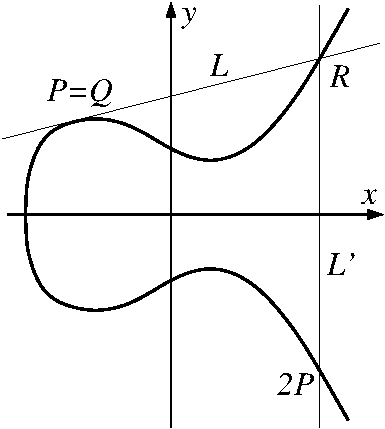
\includegraphics[scale=1.08]{ec-mult2.pdf}
\caption{Doubling the point P} \vspace{\floatsep} \vskip +20 pt
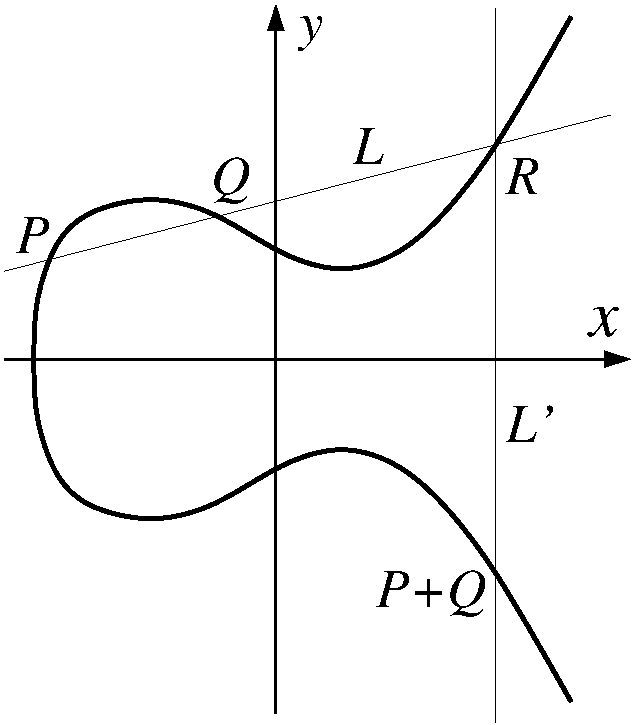
\includegraphics[scale=0.65]{ec-add.pdf}
\caption{ Adding distinct points P and Q} % \footnotemark}
\end{center}
\end{figure}
% \addtocounter{footnote}{0}\footnotetext{The point $O$ cannot be represented in the affine plane.}
\enlargethispage{+20pt}

\newpage
We must note that ${\bf E}$ can have the following meanings:
\begin{itemize}
   \item the set ${\bf E}$ of solutions pairs $(x,y)$ for an equation including the point $O$
   \item the group ${\bf E}$ (with the operation ''addition of $(x_1,y_1)$ and $(x_2,y_2)$'')
   \item the elliptic curve ${\bf E}$ (which is actually the same as the group ${\bf E}$)
\end{itemize}
For cryptography, the important fact is that, for very large numbers, it appears to be extremely difficult to use a
given point $Q$ on an elliptic curve to determine which two points have to be added to obtain $Q$.

For large numbers $a, b$ and $p$ ($p$, for example, has a length of more than $160$ bits), the computer can easily add
the point $P$  $m$ times after another, i.e. to determine the point $P + P + \cdots + P = Q$ in an incredibly short space
of time (in a few fractions of a second) ($m$ summands $P$). Rather than $P + P + \cdots + P = Q$ ($m$ summands $P$)
we also write $mP = Q$. If we have a point $P$ and a point $Q$, which both lie on the same elliptic curve, no procedure
is known that enables us --- within an acceptable space of time --- to determine the number $m$ (assuming it actually exists)
for which $mP = Q$. This is referred to as the ''elliptic curve discrete logarithm problem'' (abbreviated to ECDLP)\index{ECDLP}.

We must note that not all elliptic curves are equally secure. This
means that we must choose the parameters $a$ and $b$ carefully
when defining a curve. For certain classes of elliptic curves, it
is possible to solve the ECDLP easier than in the general case.
Cryptographically unsuitable elliptic curves are called {\em abnormal}
curves (these are curves over ${\mathbb Z}_p$ for which the set
${\bf E}$ has precisely $p$ elements) and the {\em supersingular} curves
(the curves for which we can reduce the calculation of the ECDLP
to calculating the ''standard'' discrete logarithm in other finite
fields, i.e. simplify the calculation). There are therefore
cryptographically good and bad curves. However, for given
parameters $a$ and $b$ we can, with some difficulty, establish
whether or not the resulting elliptic curve is useful for
cryptographic purposes. The curves used in cryptography are
usually provided by experts. They ensure that the elliptic curves
they classify as secure satisfy the current security requirements.

For secure curves, the parameter $p$ determines how long it takes
to solve the ECDLP on this curve. The larger the parameter $p$,
the longer it takes to solve the problem. Experts recommend a bit
length of over $200$ bits for the parameter $p$. This makes it
clear why elliptic curves are so interesting for cryptography.
Because the parameter $p$ also determines the time required to
perform the signature/encryption procedure when using elliptic
curves in cryptography. The time taken to generate a pair of keys
also depends on $p$. Thus, small values (few bits) are desirable
here (in order to minimise the run times for the procedures);
however, the required security must still be maintained. For
example, with a length of $200$ bits for $p$, a {\em good}
elliptic curve is just as secure as an \index{RSA!module} RSA
module of over $1024$ bits in length (at least according to the
current state of research). The reason for this is that the
quickest algorithms for solving the {\em elliptic curve discrete
logarithm} problem have an exponential run time --- unlike the
subexponential run times that the best factorisation algorithms
currently have (number sieve, quadratic sieve or factorisation
with elliptic curves). Therefore, the parameters for cryptographic
procedures based on the problem of {\em factorising whole numbers}
must be greater than the parameters for cryptographic procedures
based on the ECDLP problem.

\subsubsection{Digital signatures using elliptic curves}

The {\em elliptic curve discrete logarithm problem} (ECDLP) \index{ECDLP} forms the basis for
elliptic-curve cryptography. Various signature procedures are based on this.
What they have in common is how they use the public parameters and how these
parameters are used to generate secret and public keys:
\begin{itemize}
    \item The parameters of the elliptic curve E, i.e. a prime number $p$ that
determines over which field ${\mathbb Z}_p$ the elliptic curve ${\bf E}$ is
defined, as well as the two numbers $a$ and $b$ in ${\mathbb Z}_p$.
    \item A point $G=(x,y)$ that lies on the elliptic curve ${\bf E}$.
    \item A prime number $r < p$ for which $rG=O$ (i.e. $G$ added $r$ times
gives the neutral element of the group ${\bf E}$) and $r$ is a factor of $\#{\bf
E}$ (where $\# {\bf E}$ is the number of elements in the set ${\bf E}$). The
point $G$ therefore has the order $r$ and is the generator of a cyclic subgroup
of ${\bf E}$ with the order $r$.
    \item The number $k = \#{\bf E}/r$ ($k$ is called the {\em cofactor}).
\end{itemize}
The parameters $a, b, p, G, r$ and $k$ listed above are called
{\em domain parameters}.\index{Domain parameters} They determine on which elliptic curve ${\bf
E}$ and in which cyclic subgroup of ${\bf E}$ a signature
procedure has been ''used''.

The secret key $s$ of the signature generator is a (random) whole number $s$ in
the interval $[1, r-1]$. The public key of the signature generator is a point
$W=(x,y)$ on the elliptic curve ${\bf E}$. The public key $W$ and secret key $s$
are interrelated as follows: $W = sG$. This means that the domain parameters
(particularly $G$) and the secret key $s$ are used to calculate the public key
$W$ (by adding $G$ $s$ times on ${\bf E}$). The ECDLP is obviously used here: If
$W$ and $G$ (as well as the other domain parameters used) are known, then it is
difficult to use these to calculate $s$. (If the parameters are chosen
correctly, this currently appears to be practically impossible).

In order to verify a signature, the recipient of the signature must know the
following:
\begin{enumerate}
   \item The signature procedure used,
   \item The hash function used,
   \item The domain parameters used to generate the signature
   \item The public key $W$ of the signature generator.
\end{enumerate}


\subsubsection{Faktorisation using elliptic curves}

\hypertarget{faktell}{}

There are factorisation algorithms based on elliptic curves\footnote{In 1987 H.W. Lenstra published
a factorisation algorithm, based on elliptic curves (see \cite{Lenstra1987}).
The biggest compound number curently factorised with elliptic curves is the number $ 628^{59}-1, $ which has 55 decimal digits. It was
found Oct. 6th, 2001 by M. Izumi (See \hyperlink{Lenstra2}{ECMNET}\index{ECMNET}).
}. More precisely,
these procedures exploit the fact that elliptic curves can be defined over
${\mathbb Z}_n$ ($n$ composite number). Elliptic curves over ${\mathbb Z}_n$ do
not form a group, because not every point on such an elliptic curve has an
inverse point. This is connected with the fact that - if $n$ is a composite
number - there exist elements in ${\mathbb Z}_n$ that do not have an inverse
with respect to multiplication mod $n$. In order to add two points on an
elliptic curve over ${\mathbb Z}_n$, we can calculate in the same way as on
elliptic curves over ${\mathbb Z}_p$. Addition of two points (on an elliptic
curve over ${\mathbb Z}_n$), however, fails if and only if a factor of $n$ has
been found. The reason for this is that the procedure for adding points on
elliptic curves gives elements in ${\mathbb Z}_n$ and calculates the inverse
elements for these (with respect to multiplication mod $n$) in ${\mathbb Z}_n$.
The extended \index{Euclidean algorithm} Euclidean algorithm is used here. If
the addition of two points (that lie of an elliptic curve over ${\mathbb Z}_n$)
gives an element in ${\mathbb Z}_n$ that does not have an inverse element in
${\mathbb Z}_n$, then the extended Euclidean algorithm delivers a genuine factor
of $n$.

Factorisation using elliptic curves thus principally works as follows: You
select random curves over ${\mathbb Z}_n$, as well as random points (that lie on
this curve) and add them; you thus obtain points that also lie on the curve or
find a factor of $n$. Factorisation algorithms based on elliptic curves
therefore work probabilistically. The opportunity of defining large number of
elliptic curves over ${\mathbb Z}_n$ allows you to increase the probability of
finding two points which you can add to obtain a factor of $n$. These procedures
are therefore highly suitable for parallelisation.

\subsection{Implementing elliptic curves}

CrypTool uses elliptic curves for the digital signature function.

It implements the basic algorithms for group operations, for generating elliptic
curves, for importing and exporting parameters for elliptic curves over finite
fields with $p$ ($p$ prime) elements. The algorithms have been implemented in
ANSI C and comply with draft no. 8 of the IEEE P1363 work group {\em Standard
Specifications for Public Key Cryptography}

{\href{http://grouper.ieee.org/groups/1363}{\tt
http://grouper.ieee.org/groups/1363}}.

The procedure implements the cryptographic primitives for generating and
verifying signatures for the variations of Nyberg-Rueppel signatures and
\index{DSA} DAS signatures based on elliptic curves (in accordance with draft
no. 8 of the IEEE P1363 work group). This was done in collaboration with the
SECUDE GmbH --- using the above library and the SECUDE SDK.
\index{SECUDE GmbH}

\newpage
%\addcontentsline{toc}{subsection}{Literaturverzeichnis}
\begin{thebibliography}{99999}
\addcontentsline{toc}{subsection}{Bibliography}
	\bibitem[Lenstra1987]{Lenstra1987} H.W. Lenstra\\ \index{Lenstra 1987}
		Factoring integers with elliptic curves, Annals of Mathematics 126, pp. 649-673, 1987.
\end{thebibliography}
%\newpage

\section*{URLs}\addcontentsline{toc}{subsection}{URLs}

\begin{enumerate}
   \item Certicom � Online Tutorial, \index{Certicom}\\
		\href{http://www.certicom.com/resources/ecc_tutorial/ecc_tutorial.html}{\tt http://www.certicom.com/resources/ecc\_tutorial/ecc\_tutorial.html}
	\item IEEE P1363

		\href{http://grouper.ieee.org/groups/1363}{\tt http://grouper.ieee.org/groups/1363}
	\item  \hypertarget{Lenstra2}{}
An informative web page to the factorisation with elliptic curves.

\href{http://www.loria.fr/~zimmerma/records/ecmnet.html}{\tt http://www.loria.fr/\~{}zimmerma/records/ecmnet.html}

There, one finds literature to the topic factorisation with elliptic curves as well as link to other web page. 

\end{enumerate}

\addcontentsline{toc}{section}{Index} 
\printindex
%
% ......................................................................................................................
%
% ~~~~~~~~~~~~~~~~~~~~~~~~~~~~~~~~~~~~~~~~~~~~~~~~~~~~~~~~~~~~~~~~~~~~~~~~~~~~~~~~~~~~~~~~~~~~~~~~~~~~~~~~~~~~~~~~~~~~~~
%

\end{document}


